%===============================================================
% RAPPORT DE FIN D'ETUDES - ESPRIT 2025-2026
% Maryem Achoury - Genie Logiciel - LinSoft
%===============================================================
\documentclass[12pt,a4paper]{report}

\usepackage[utf8]{inputenc}
\usepackage[T1]{fontenc}
\usepackage{mathptmx}
\usepackage[top=2.5cm,bottom=2.5cm,left=2.5cm,right=2.5cm]{geometry}
\usepackage{setspace}
\setstretch{1.15}
\usepackage{parskip}
\setlength{\parindent}{0.5cm}
\usepackage{graphicx}
\usepackage{float}
\usepackage{array}
\usepackage{longtable}
\usepackage{tabularx}
\usepackage{multirow}
\usepackage{colortbl}
\usepackage[table]{xcolor}
\usepackage{fancyhdr}
\setlength{\headheight}{14pt}
\usepackage{titlesec}
\usepackage{tocloft}
\usepackage{hyperref}
\usepackage{caption}
\usepackage{enumitem}
\usepackage{amsmath}
\usepackage{listings}
\usepackage{pdfpages}
\usepackage{emptypage}
\usepackage{microtype}
\usepackage{booktabs}

% --- Noms francais manuels (sans babel) ---
\AtBeginDocument{
  \renewcommand{\chaptername}{Chapitre}
  \renewcommand{\contentsname}{Table des mati\`eres}
  \renewcommand{\listfigurename}{Liste des figures}
  \renewcommand{\listtablename}{Liste des tableaux}
  \renewcommand{\bibname}{Bibliographie}
  \renewcommand{\figurename}{Figure}
  \renewcommand{\tablename}{Tableau}
}

% --- Palette de couleurs ---
\definecolor{espritBlue}{RGB}{0,84,166}
\definecolor{lightBlue}{RGB}{217,230,243}
\definecolor{headerGray}{RGB}{89,89,89}
\definecolor{codeGray}{RGB}{245,245,245}
\definecolor{accentRed}{RGB}{192,0,0}
\definecolor{darkGreen}{RGB}{21,87,36}
\definecolor{lightGreen}{RGB}{212,237,218}

% --- Hyperref ---
\hypersetup{
  colorlinks=true,
  linkcolor=espritBlue,
  urlcolor=espritBlue,
  citecolor=espritBlue,
  pdftitle={Rapport PFE -- Maryem Achoury -- LinSoft 2025/2026},
  pdfauthor={Maryem Achoury},
  pdfsubject={Microservices, IA, Gestion d'evenements, OpenShift}
}

% --- En-tetes ---
\pagestyle{fancy}
\fancyhf{}
\fancyhead[L]{\small\textcolor{headerGray}{PFE -- Maryem Achoury | LinSoft -- 2025/2026}}
\fancyhead[R]{\small\textcolor{headerGray}{\leftmark}}
\fancyfoot[C]{\thepage}
\renewcommand{\headrulewidth}{0.4pt}

% --- Formatage des titres ---
\titleformat{\chapter}[display]
  {\normalfont\huge\bfseries\color{espritBlue}}
  {\chaptertitlename\ \thechapter}{20pt}{\Huge}
\titlespacing*{\chapter}{0pt}{0pt}{40pt}
\titleformat{\section}{\normalfont\Large\bfseries\color{espritBlue}}{\thesection}{1em}{}
\titleformat{\subsection}{\normalfont\large\bfseries\color{headerGray}}{\thesubsection}{1em}{}
\titleformat{\subsubsection}{\normalfont\normalsize\bfseries\color{espritBlue}}{\thesubsubsection}{1em}{}

% --- Listings Python ---
\lstset{
  backgroundcolor=\color{codeGray},
  basicstyle=\ttfamily\footnotesize,
  breaklines=true,
  frame=single,
  rulecolor=\color{gray},
  keywordstyle=\color{espritBlue}\bfseries,
  commentstyle=\color{headerGray}\itshape,
  stringstyle=\color{accentRed},
  numbers=left,
  numberstyle=\tiny\color{gray},
  numbersep=6pt,
  showstringspaces=false,
  tabsize=2,
  captionpos=b
}

% --- Types de colonnes ---
\newcolumntype{L}[1]{>{\raggedright\arraybackslash}p{#1}}
\newcolumntype{C}[1]{>{\centering\arraybackslash}p{#1}}
\newcolumntype{R}[1]{>{\raggedleft\arraybackslash}p{#1}}
\arrayrulecolor{gray}

% --- En-tete de tableau colore ---
\newcommand{\tH}[1]{\cellcolor{lightBlue}\textbf{#1}}

% --- Boite mise en evidence ---
\newcommand{\highlight}[1]{%
  \noindent\colorbox{lightGreen}{\parbox{\dimexpr\linewidth-2\fboxsep}{%
    \textcolor{darkGreen}{\textbf{#1}}}}%
}

% --- Badge technologie (remplacer par \includegraphics quand logo disponible) ---
\newcommand{\techbadge}[1]{%
  \fcolorbox{espritBlue}{lightBlue}{%
    \parbox[c][1cm][c]{2.2cm}{\centering
      \textcolor{espritBlue}{\footnotesize\textbf{#1}}%
    }%
  }%
}

% --- Placeholder pour images en attente ---
\newcommand{\placeholder}[2][0.88\textwidth]{%
  \begin{center}
  \setlength{\fboxsep}{0pt}%
  \fcolorbox{espritBlue}{lightBlue}{%
    \parbox{#1}{\vspace{1.8cm}\centering
      \textcolor{espritBlue}{\large\textbf{#2}}\\[0.4cm]
      \textcolor{headerGray}{\small\itshape (ins\'erer l'image correspondante)}
      \vspace{1.8cm}
    }%
  }
  \end{center}
}

%==================================================================
\begin{document}
%==================================================================

%------------------------------------------------------------------
% PAGE DE GARDE
%------------------------------------------------------------------
\begin{titlepage}
\pagestyle{empty}
\begin{center}

\begin{minipage}{0.42\textwidth}
  \centering
  \fcolorbox{espritBlue}{white}{%
    \parbox[c][2cm][c]{5cm}{\centering
      \textcolor{espritBlue}{\LARGE\textbf{ESPRIT}}\\[0.2cm]
      \textcolor{headerGray}{\footnotesize\'Ecole Sup\'erieure Priv\'ee\\
      d'Ing\'enierie et de Technologies}
    }%
  }
\end{minipage}
\hfill
\begin{minipage}{0.42\textwidth}
  \centering
  \fcolorbox{espritBlue}{white}{%
    \parbox[c][2cm][c]{5cm}{\centering
      \textcolor{espritBlue}{\LARGE\textbf{LinSoft}}\\[0.2cm]
      \textcolor{headerGray}{\footnotesize Soci\'et\'e de Services\\
      en Ing\'enierie Informatique}
    }%
  }
\end{minipage}

\vspace{0.4cm}
\noindent\rule{\linewidth}{0.5pt}
\vspace{0.2cm}

{\small\textbf{R\'epublique Tunisienne}}\\
{\small\textbf{Minist\`ere de l'Enseignement Sup\'erieur et de la Recherche Scientifique}}\\[0.4cm]
{\large\textbf{ESPRIT -- \'Ecole Sup\'erieure Priv\'ee d'Ing\'enierie et de Technologies}}\\[0.2cm]
{\normalsize D\'epartement G\'enie Logiciel}\\[0.3cm]

\noindent\rule{\linewidth}{0.5pt}\\[0.3cm]

{\LARGE\textbf{RAPPORT DE PROJET DE FIN D'\'ETUDES}}\\[0.4cm]

\noindent\rule{\linewidth}{1.5pt}\\[0.5cm]

\begin{minipage}{\textwidth}
\centering
{\Large\textbf{Automatisation et optimisation de la gestion\\[0.25cm]
d'\'ev\'enements via une architecture microservices\\[0.25cm]
avec Intelligence Artificielle et d\'eploiement sur OpenShift}}
\end{minipage}

\vspace{0.5cm}
\noindent\rule{\linewidth}{1.5pt}\\[0.8cm]

\begin{tabular}{@{}ll@{}}
  \textbf{R\'ealis\'ee par :}            & Maryem Achoury \\[0.5cm]
  \textbf{Encadrant acad\'emique :}      & [\`A compl\'eter] \\[0.5cm]
  \textbf{Encadrant professionnel :}     & [\`A compl\'eter] \\[0.5cm]
  \textbf{Entreprise d'accueil :}        & LinSoft \\[0.5cm]
  \textbf{Sp\'ecialit\'e :}             & G\'enie Logiciel \\
\end{tabular}

\vfill

\noindent\rule{\linewidth}{0.5pt}\\[0.3cm]
{\large\textbf{Ann\'ee universitaire 2025 -- 2026}}

\end{center}
\end{titlepage}

%------------------------------------------------------------------
% FORMULAIRE DE VALIDATION DU DEPOT
%------------------------------------------------------------------
\newpage
\thispagestyle{empty}
\vspace*{0.5cm}

\begin{center}
{\large\textbf{Je valide le d\'ep\^ot du rapport PFE relatif \`a l'\'etudiant nomm\'e ci-dessous}}\\[0.3cm]
{\itshape I validate the submission of the student's report:}
\end{center}

\bigskip
\noindent\textbf{Nom \& Pr\'enom / Name \& Surname :}\quad
\underline{\hspace{8cm}}

\vspace{1.5cm}

\begin{table}[H]
\centering
\renewcommand{\arraystretch}{1}
\begin{tabular}{|p{7.2cm}|p{7.2cm}|}
\hline
\vspace{0.3cm}\textbf{Encadrant Entreprise / Business Supervisor}\\[0.3cm]
Nom \& Pr\'enom : \dotfill\\[0.5cm]
\vspace{3.5cm}
Cachet \& Signature :
&
\vspace{0.3cm}\textbf{Encadrant Acad\'emique / Academic Supervisor}\\[0.3cm]
Nom \& Pr\'enom : \dotfill\\[0.5cm]
\vspace{3.5cm}
Signature :
\\[3cm]
\hline
\end{tabular}
\end{table}

\vspace{1.5cm}
\begin{center}
{\small\itshape
Ce formulaire doit \^etre rempli, sign\'e et scann\'e /
\textbf{This form must be completed, signed and scanned.}\\[0.2cm]
Ce formulaire doit \^etre introduit apr\`es la page de garde /
This form must be inserted after the cover page.}
\end{center}

%------------------------------------------------------------------
% PAGES LIMINAIRES
%------------------------------------------------------------------
\newpage
\pagestyle{plain}
\pagenumbering{roman}

%--- RESUME -------------------------------------------------------
\chapter*{R\'esum\'e}
\addcontentsline{toc}{chapter}{R\'esum\'e}

Ce projet de fin d'\'etudes, men\'e au sein de la soci\'et\'e LinSoft sur une p\'eriode de six mois,
avait pour objectif de pallier les insuffisances du syst\`eme de gestion d'\'ev\'enements en place
-- une simple page web statique sans fonctionnalit\'es interactives -- en concevant et
d\'eveloppant une plateforme compl\`ete, intelligente et scalable.

La solution propos\'ee s'appuie sur une \textbf{architecture microservices} compos\'ee de six
services ind\'ependants d\'eploy\'es sur \textbf{OpenShift} : \textit{events-service},
\textit{registrations-service}, \textit{users-service}, \textit{notifications-service},
\textit{dashboard-service} et \textit{charges-service}. L'int\'egrit\'e du syst\`eme repose sur
trois piliers techniques : un bus de messages \textbf{Apache Kafka} pour la communication
asynchrone inter-services, un serveur d'identit\'e \textbf{Keycloak} pour la s\'ecurisation
centralis\'ee via OAuth2/OIDC, et une base de donn\'ees \textbf{MongoDB} par service
(pattern \textit{Database-per-Service}). Le backend est d\'evelopp\'e avec \textbf{Quarkus}
(Java), les interfaces avec \textbf{Angular} (BackOffice) et \textbf{React} (FrontOffice).

La contribution la plus distinctive de ce projet r\'eside dans le \textit{charges-service},
qui impl\'emente un triple m\'ecanisme : gestion d'un catalogue de ressources, affectation des
charges avec calcul automatique du co\^ut pr\'evisionnel, et pr\'ediction du budget global par un
mod\`ele \textbf{Random Forest} (scikit-learn). Ce double calcul -- direct et IA -- offre \`a
l'organisateur un outil de pilotage budg\'etaire sans \'equivalent dans les solutions du march\'e.

\medskip
\noindent\textbf{Mots-cl\'es :} Microservices, Quarkus, Angular, React, MongoDB, Apache Kafka,
Keycloak, OAuth2/OIDC, OpenShift, Docker, Intelligence Artificielle, Random Forest,
Pr\'ediction des co\^uts, Gestion d'\'ev\'enements.

\bigskip

\chapter*{Abstract}
\addcontentsline{toc}{chapter}{Abstract}

This final-year project, carried out at LinSoft over a six-month internship, aimed at
replacing an outdated static event page with a fully featured, intelligent, and cloud-native
event management platform. The solution is built on a \textbf{microservices architecture}
comprising six independently deployable services, orchestrated on \textbf{OpenShift} (Red Hat
Kubernetes). Asynchronous inter-service communication is handled by \textbf{Apache Kafka},
while identity management leverages \textbf{Keycloak} (OAuth2/OIDC). Each microservice owns
its \textbf{MongoDB} instance following the Database-per-Service pattern.

The standout feature is the \textit{charges-service}, which combines a charge catalogue,
event-level cost assignment, and an AI-powered \textbf{Random Forest} model that predicts
total event costs from macroscopic parameters (type, size, duration, location). This
dual-validation approach -- computed cost vs.\ predicted cost -- enables precise budgetary
control that no off-the-shelf solution currently offers.

\medskip
\noindent\textbf{Keywords:} Microservices, Quarkus, Angular, React, MongoDB, Apache Kafka,
Keycloak, OAuth2/OIDC, OpenShift, Docker, Artificial Intelligence, Random Forest,
Cost Prediction, Event Management.

%--- DEDICACE -----------------------------------------------------
\chapter*{D\'edicace}
\addcontentsline{toc}{chapter}{D\'edicace}

\vspace*{3cm}
\begin{center}
\itshape\large
\`A mes parents,\\
dont le soutien indef\'ectible a \'et\'e mon ancre tout au long de ce parcours.\\[1cm]
\`A mes fr\`eres et s\oe urs,\\
pour leur bienveillance et leur encouragement quotidien.\\[1cm]
\`A mes amis et coll\`egues de promotion,\\
avec qui j'ai partag\'e les moments de doute et de victoire.\\[1cm]
\`A tous ceux qui croient que la technologie peut rendre le monde plus efficace.
\end{center}

%--- REMERCIEMENTS ------------------------------------------------
\chapter*{Remerciements}
\addcontentsline{toc}{chapter}{Remerciements}

Ce travail n'aurait pas \'et\'e ce qu'il est sans la contribution de nombreuses personnes que
je tiens \`a remercier sinc\`erement.

Mes premiers remerciements vont \`a mon encadrant acad\'emique, dont les remarques
constructives et la rigueur intellectuelle m'ont aid\'ee \`a progresser dans la formalisation
des concepts et dans la qualit\'e de la r\'edaction.

Je suis \'egalement tr\`es reconnaissante envers l'\'equipe technique de \textbf{LinSoft}, et plus
particuli\`erement mon encadrant professionnel, pour la confiance accord\'ee d\`es le premier
jour, la libert\'e de conception laiss\'ee dans les choix d'architecture, et les nombreuses
heures de revue de code qui ont fait maturier ce projet.

Je remercie enfin le corps professoral d'ESPRIT pour la formation solide en ing\'enierie
logicielle qui m'a donn\'e les outils conceptuels n\'ecessaires \`a l'accomplissement de ce
travail. La maitrise des architectures distribu\'ees, des patterns cloud-native et des
approches DevOps, acquise lors de mes ann\'ees d'\'etudes, a \'et\'e d\'eterminante.

%--- ABREVIATIONS -------------------------------------------------
\chapter*{Liste des abr\'eviations}
\addcontentsline{toc}{chapter}{Liste des abr\'eviations}

\begin{longtable}{L{3cm} L{11cm}}
  \hline
  \tH{Abr\'eviation} & \tH{Signification} \\
  \hline
  \endfirsthead
  \hline
  \tH{Abr\'eviation} & \tH{Signification} \\
  \hline
  \endhead
  \hline
  \endfoot
  API       & Application Programming Interface \\
  CI/CD     & Continuous Integration / Continuous Deployment \\
  CRUD      & Create, Read, Update, Delete \\
  HPA       & Horizontal Pod Autoscaler (Kubernetes) \\
  HTTP/S    & HyperText Transfer Protocol / Secure \\
  IA        & Intelligence Artificielle \\
  IAM       & Identity and Access Management \\
  JWT       & JSON Web Token \\
  MAE       & Mean Absolute Error (erreur absolue moyenne) \\
  ML        & Machine Learning \\
  NoSQL     & Not Only SQL \\
  OAuth2    & Open Authorization 2.0 \\
  OIDC      & OpenID Connect \\
  REST      & Representational State Transfer \\
  RF        & Random Forest \\
  RBAC      & Role-Based Access Control \\
  SPA       & Single Page Application \\
  SSII      & Soci\'et\'e de Services en Ing\'enierie Informatique \\
  SSO       & Single Sign-On \\
  TDD       & Test-Driven Development \\
  TLS       & Transport Layer Security \\
  UML       & Unified Modeling Language \\
  \hline
\end{longtable}

%--- TABLE DES MATIERES -------------------------------------------
\tableofcontents
\listoffigures
\listoftables
\newpage

%==================================================================
% CORPS DU RAPPORT
%==================================================================
\cleardoublepage
\pagestyle{fancy}
\pagenumbering{arabic}

%==================================================================
\chapter*{Introduction g\'en\'erale}
\addcontentsline{toc}{chapter}{Introduction g\'en\'erale}
\markboth{Introduction g\'en\'erale}{}
%==================================================================

La num\'erisation des processus organisationnels constitue aujourd'hui l'un des axes
strat\'egiques prioritaires des entreprises technologiques. Dans un contexte o\`u la
v\'elocit\'e, la traitement des donn\'ees en temps r\'eel et la r\'esilience des syst\`emes sont
devenus des crit\`eres de comp\'etitivit\'e, les architectures logicielles traditionnelles
montrent leurs limites face aux exigences des usages modernes.

La gestion des \'ev\'enements professionnels -- conf\'erences, workshops, forums -- illustre
parfaitement cette tension entre les pratiques h\'erit\'ees et les besoins contemporains.
Chez LinSoft, une SSII tunisienne active dans l'int\'egration de solutions cloud et
l'organisation d'\'ev\'enements IT r\'egionaux, cette probl\'ematique s'est manifest\'ee de
mani\`ere concr\`ete : absence de syst\`eme d'inscription en ligne, gestion des ressources
mat\'erielles enti\`erement manuelle, aucun outil de projection budg\'etaire, et des
notifications assur\'ees manuellement par l'\'equipe.

C'est dans ce cadre que ce projet de fin d'\'etudes a \'et\'e initi\'e. L'objectif \'etait ambitieux :
concevoir, d\'evelopper et d\'eployer une plateforme compl\`ete de gestion d'\'ev\'enements, en
adoptant les standards actuels de l'ing\'enierie cloud -- architecture microservices,
communication asynchrone via Apache Kafka, s\'ecurisation par Keycloak, persistance
distribu\'ee MongoDB -- et en y int\'egrant un module d'intelligence artificielle pour
la pr\'ediction des co\^uts logistiques.

Le pr\'esent rapport est structur\'e en quatre chapitres compl\'ementaires :

\begin{itemize}[leftmargin=1.5cm]
  \item Le \textbf{Chapitre 1 -- \'Etude pr\'ealable} -- d\'ecrit l'organisme d'accueil, pose
  la probl\'ematique, analyse les solutions existantes sur le march\'e et d\'etaille la
  solution retenue avec sa m\'ethodologie de d\'eveloppement.
  \item Le \textbf{Chapitre 2 -- Sp\'ecification des besoins} -- pr\'esente les acteurs du
  syst\`eme, les exigences fonctionnelles et non-fonctionnelles, accompagn\'ees des
  diagrammes de cas d'utilisation et du mod\`ele de classes.
  \item Le \textbf{Chapitre 3 -- Conception} -- d\'etaille l'architecture microservices, les
  choix de communication, la mod\'elisation des flux m\'etier et la s\'ecurisation, illustr\'es
  par l'ensemble des diagrammes UML.
  \item Le \textbf{Chapitre 4 -- R\'ealisation} -- couvre l'environnement technique,
  l'impl\'ementation des services, les interfaces utilisateur et le d\'eploiement sur
  OpenShift avec les \'el\'ements de validation.
\end{itemize}

%==================================================================
\chapter{\'Etude Pr\'ealable}
%==================================================================

\section*{Introduction}
\addcontentsline{toc}{section}{Introduction}

Tout projet de d\'eveloppement logiciel s\'erieux commence par une phase d'analyse approfondie
du contexte : comprendre l'entreprise qui accueille le stagiaire, identifier avec pr\'ecision
les dysfonctionnements existants, et \'evaluer les solutions disponibles sur le march\'e avant
de formuler une proposition adapt\'ee. Ce chapitre parcourt ces \'etapes fondatrices.

%------------------------------------------------------------------
\section{Pr\'esentation de LinSoft}
%------------------------------------------------------------------

\textbf{LinSoft} est une Soci\'et\'e de Services en Ing\'enierie Informatique (SSII) fond\'ee en
Tunisie, sp\'ecialis\'ee dans l'int\'egration de solutions IT complexes pour des clients de la
r\'egion Moyen-Orient et Afrique (MEA). Positionn\'ee sur le segment haut de gamme, elle
intervient dans des domaines \`a forte valeur technique :

\begin{itemize}[noitemsep]
  \item Conception et d\'eveloppement d'applications web et mobiles ;
  \item Architecture microservices, syst\`emes distribu\'es et cloud-native ;
  \item D\'eploiement sur plateformes conteneuris\'ees (OpenShift, Kubernetes) ;
  \item Int\'egration IAM, s\'ecurisation et gestion des identit\'es ;
  \item Solutions de data engineering et d'intelligence artificielle ;
  \item Formation et certification aux technologies strat\'egiques (Quarkus, Kafka, Red Hat).
\end{itemize}

\begin{figure}[H]
  \centering
  
\includegraphics[width=0.45\textwidth]{figures/logo-linsoftt.png}
  \caption{Logo de la soci\'et\'e LinSoft}
  \label{fig:logo_linsoft}
\end{figure}

LinSoft organise r\'eguli\`erement des \'ev\'enements IT d'envergure -- conf\'erences techniques,
workshops de certification, participation au GITEX Afrique -- qui rassemblent des centaines
de participants. Ces \'ev\'enements, essentiels pour la visibilit\'e et le rayonnement de
l'entreprise, \'etaient pourtant g\'er\'es avec des outils n\'etant pas \`a la hauteur des ambitions
de la soci\'et\'e.

%------------------------------------------------------------------
\section{Probl\'ematique}
%------------------------------------------------------------------

L'observation du fonctionnement interne de LinSoft a permis d'identifier plusieurs
dysfonctionnements concrets dans la gestion de ses \'ev\'enements :

\begin{enumerate}[leftmargin=1.5cm]
  \item \textbf{Absence totale d'inscription en ligne} : les participants devaient contacter
  LinSoft par email ou t\'el\'ephone, g\'en\'erant un traitement manuel fastidieux et source d'erreurs.
  \item \textbf{Aucun suivi en temps r\'eel} : aucun outil ne permettait de conna\^itre
  instantan\'ement le nombre d'inscrits, les listes d'attente, ou le taux de remplissage.
  \item \textbf{Notifications manuelles} : les confirmations d'inscription et les rappels
  \'etaient envoy\'es manuellement, sans coh\'erence ni automatisation.
  \item \textbf{Gestion des ressources absente} : les besoins mat\'eriels (projecteurs, tables,
  traiteur, microphones) \'etaient estim\'es \`a la louche, sans catalogue ni traitement structur\'e.
  \item \textbf{Budget empirique} : sans outil de calcul, les co\^uts \'etaient sous-estim\'es ou
  sur-estim\'es, rendant le pilotage budg\'etaire impossible.
\end{enumerate}

Ces lacunes engendraient des pertes de temps significatives, des risques d'erreurs humaines
r\'ep\'et\'ees et une incapacit\'e \`a monter en charge lors des grands \'ev\'enements. La
n\'ecessit\'e d'une solution num\'erique int\'egr\'ee s'est impos\'ee comme une priorit\'e
op\'erationnelle.

%------------------------------------------------------------------
\section{\'Etude de l'existant}
%------------------------------------------------------------------

\subsection{Le syst\`eme actuel de LinSoft}

LinSoft disposait, au moment de d\'emarrer ce projet, d'une page d\'edi\'ee aux \'ev\'enements
sur son site institutionnel (\url{linsoft.com/fr/events}), sous le slogan
\textit{``Inspirez-vous. Connectez-vous. \'Evoluez.''}. Cette page se limitait \`a lister
les \'ev\'enements pass\'es et \`a venir, sans aucune interaction possible :

\begin{itemize}[noitemsep]
  \item \textbf{Pas d'inscription} : aucun formulaire, aucun bouton d'action ;
  \item \textbf{Pas de gestion} : les \'ev\'enements \'etaient cr\'e\'es directement dans le CMS,
  sans workflow d'approbation ni gestion de statut ;
  \item \textbf{Pas de donn\'ees} : LinSoft ne disposait d'aucune donn\'ee structur\'ee sur ses
  participants, leur provenance ou leur comportement.
\end{itemize}

\begin{figure}[H]
  \centering
  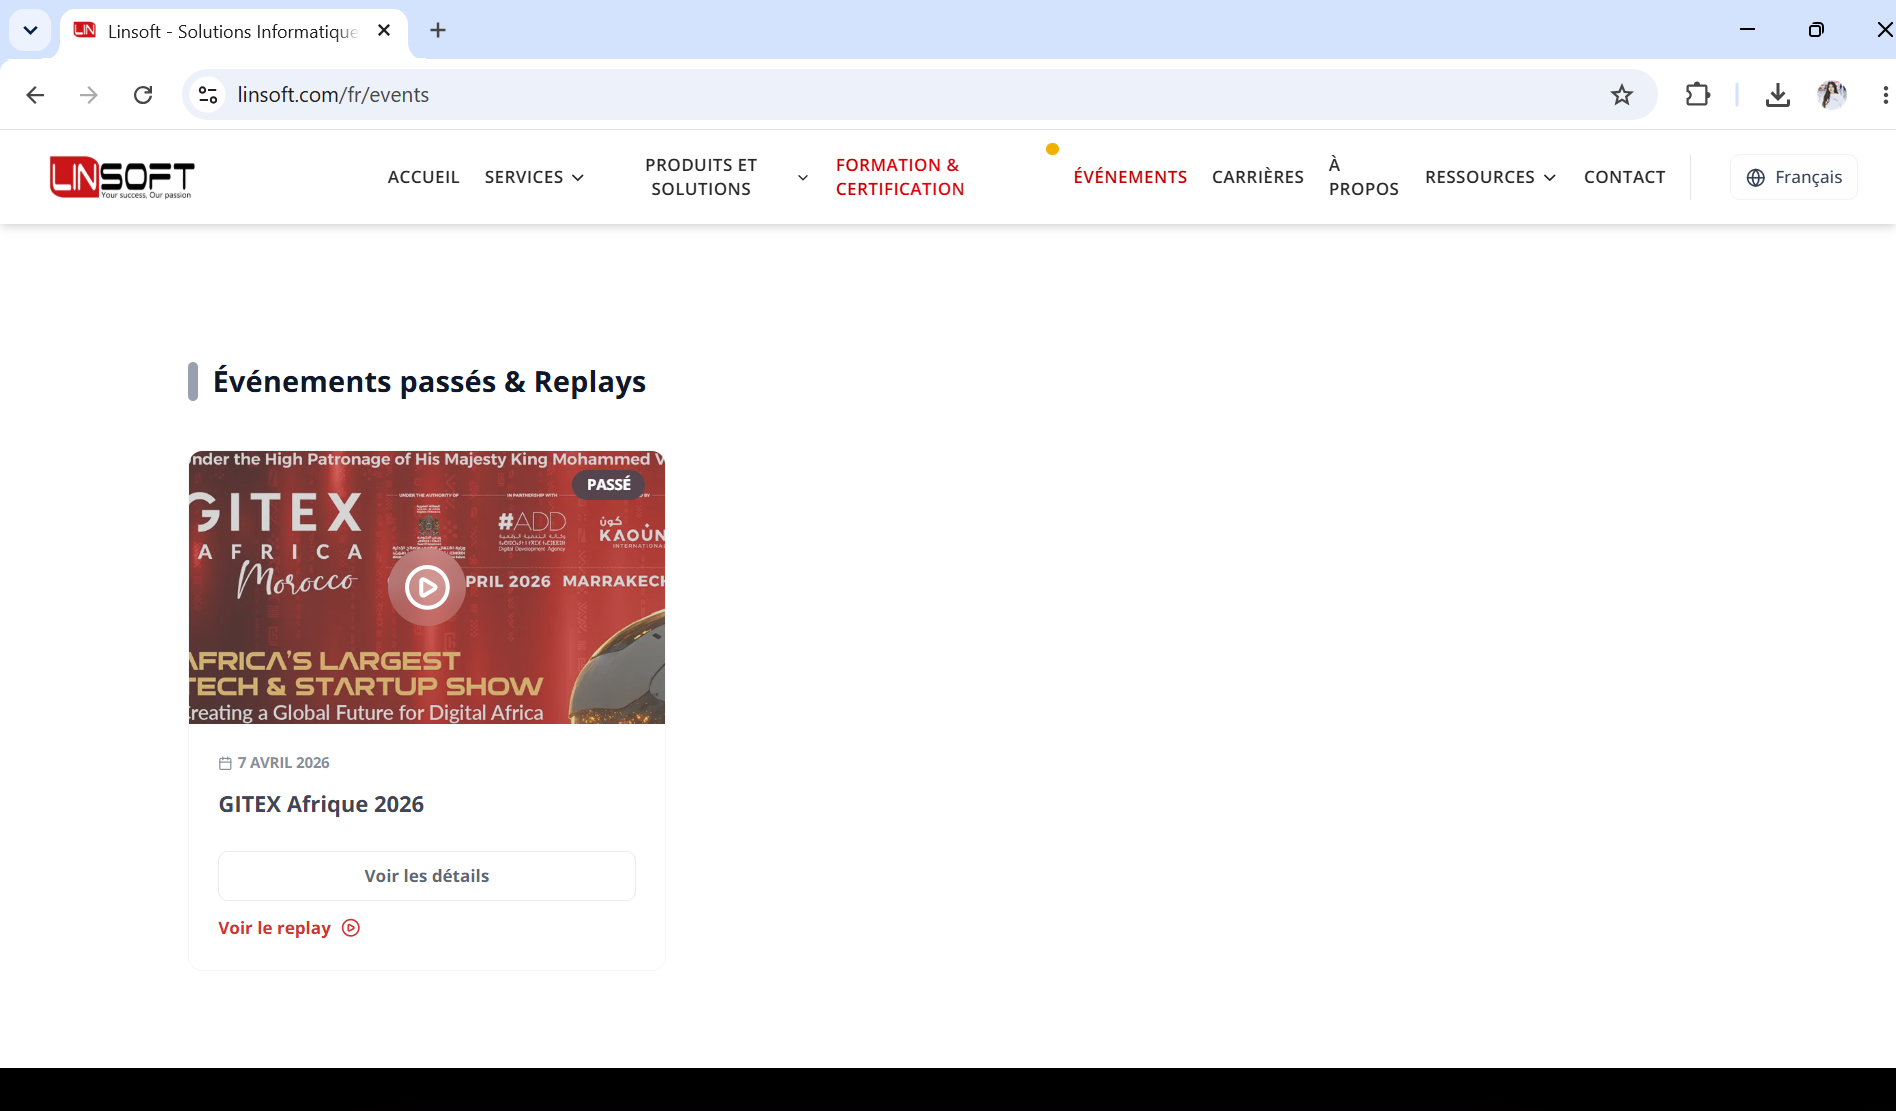
\includegraphics[width=0.92\textwidth]{figures/linsoft_event.png}
  \caption{Capture de la page \'ev\'enements existante -- \texttt{linsoft.com/fr/events}}
  \label{fig:linsoft_event}
\end{figure}

\subsection{Analyse des solutions du march\'e}

Plusieurs plateformes existent pour la gestion d'\'ev\'enements. Leur \'etude comparée a mis en
\'evidence des limitations dans le contexte sp\'ecifique de LinSoft :

\begin{table}[H]
\centering
\caption{Analyse comparative des solutions du march\'e}
\label{tab:comparaison}
\renewcommand{\arraystretch}{1.5}
\begin{tabularx}{\textwidth}{L{2.8cm} L{4.5cm} L{5.5cm}}
\hline
\tH{Solution} & \tH{Points forts} & \tH{Limites pour LinSoft} \\
\hline
Eventbrite     & Inscription en ligne, paiement & Pas de module charges/IA, RGPD non adapt\'e, co\^ut \'elev\'e \\
\hline
Meetup         & Communaut\'es, r\'ecurrence & Orient\'e grand public, RBAC limit\'e, pas de gestion budg\'etaire \\
\hline
Google Forms   & Simplicite, gratuit & Pas de gestion de capacit\'e, pas d'automatisation, no tracking \\
\hline
D\'eveloppement maison ant\'erieur & Personnalisable & Monolithique, non scalable, maintenance difficile \\
\hline
\textbf{Notre solution} & Microservices, IA, Kafka, OpenShift & Sp\'ecifique LinSoft, enti\`erement personnalis\'ee \\
\hline
\end{tabularx}
\end{table}

Cette comparaison justifie le choix d'un d\'eveloppement sur mesure : aucune solution
existante ne couvrait simultan\'ement la gestion des charges mat\'erielles, la pr\'ediction
des co\^uts par IA, et la scalabilit\'e cloud requise.

\subsection{Synth\`ese des besoins identifi\'es}

\begin{table}[H]
\centering
\caption{Besoins identifi\'es et solutions cibles}
\label{tab:besoins}
\renewcommand{\arraystretch}{1.4}
\begin{tabularx}{\textwidth}{L{4cm} L{4cm} L{5.5cm}}
\hline
\tH{Besoin} & \tH{Situation actuelle} & \tH{Solution cible} \\
\hline
Inscription en ligne    & Canal externe (email) & Formulaire + confirmation automatique \\
\hline
Suivi participants      & Non centralis\'e      & Dashboard temps r\'eel (Kafka) \\
\hline
Notifications           & Manuelles             & Email/SMS automatis\'es via Kafka \\
\hline
Gestion des charges     & Absente               & Catalogue + affectation + total \\
\hline
Pr\'ediction co\^uts   & Empirique             & Random Forest scikit-learn \\
\hline
Scalabilit\'e          & Site monolithique     & Microservices + OpenShift HPA \\
\hline
S\'ecurit\'e           & Basique               & Keycloak OAuth2/OIDC, JWT \\
\hline
\end{tabularx}
\end{table}

%------------------------------------------------------------------
\section{Solution propos\'ee}
%------------------------------------------------------------------

\subsection{Vision g\'en\'erale}

La solution propos\'ee est une plateforme cloud-native de gestion d'\'ev\'enements,
con\c{c}ue autour de six microservices autonomes communicant via REST (synchrone) et
Apache Kafka (asynchrone). Elle repose sur les principes suivants :

\begin{itemize}[noitemsep]
  \item \textbf{S\'eparation des responsabilit\'es} (Single Responsibility) : chaque service
  couvre un domaine m\'etier pr\'ecis et d\'eploy\'e ind\'ependamment ;
  \item \textbf{Base de donn\'ees par service} (Database-per-Service) : chaque microservice
  poss\`ede son instance MongoDB, garantissant l'isolation totale des donn\'ees ;
  \item \textbf{Communication pilot\'ee par \'ev\'enements} (Event-Driven) : les actions m\'etier
  g\'en\`erent des \'ev\'enements Kafka consomm\'es de mani\`ere asynchrone ;
  \item \textbf{S\'ecurisation centralis\'ee} : un serveur Keycloak unique g\`ere l'authentification
  et les autorisations pour tous les services.
\end{itemize}

\subsection{Microservices de la plateforme}

\begin{table}[H]
\centering
\caption{Description des six microservices}
\label{tab:services}
\renewcommand{\arraystretch}{1.5}
\begin{tabularx}{\textwidth}{L{3.5cm} C{1.5cm} L{8.5cm}}
\hline
\tH{Microservice} & \tH{Port} & \tH{Responsabilit\'es} \\
\hline
events-service         & 8081 & Cr\'eation, publication, modification et cycle de vie des \'ev\'enements \\
\hline
registrations-service  & 8082 & Inscriptions, listes d'attente, gestion des places disponibles \\
\hline
users-service          & 8083 & Comptes utilisateurs, profils, synchronisation avec Keycloak \\
\hline
notifications-service  & 8084 & Email et SMS automatis\'es, pilot\'es par consommation Kafka \\
\hline
dashboard-service      & 8085 & Agr\'egation de statistiques en temps r\'eel, exports \\
\hline
charges-service        & 8086 & Catalogue de charges, affectation, calcul budg\'etaire et pr\'ediction IA \\
\hline
\end{tabularx}
\end{table}

\subsection{M\'ethodologie de d\'eveloppement}

\subsubsection*{M\'ethode de gestion de projet : Agile Scrum}

Pour r\'ealiser notre projet, nous avons choisi d'utiliser le cadre de travail \textbf{SCRUM},
dont la structure favorise les r\'eunions quotidiennes (\textit{Daily Stand-up}), ce qui renforce
la communication entre les membres de l'\'equipe et contribue \`a instaurer une atmosph\`ere
de travail collaborative. Cette dynamique de groupe augmente le rendement collectif et, par
cons\'equent, acc\'el\`ere l'avancement du projet tout en am\'eliorant la qualit\'e livr\'ee.

En outre, SCRUM nous a permis de mieux respecter les d\'elais planifi\'es pour chacune des
parties du projet. Son principe central consiste \`a concentrer l'\'equipe de d\'eveloppement
sur un ensemble de fonctionnalit\'es \`a r\'ealiser de fa\c{c}on it\'erative, dans des it\'erations
de deux semaines appel\'ees \textbf{Sprints}. Chaque Sprint aboutit \`a la livraison d'un
incrément fonctionnel, testable et int\'egrable dans la solution globale.

\paragraph{D\'eroulement des sprints.}
Le backlog produit a \'et\'e maintenu sur \textbf{Jira}, avec des d\'eploiements continus
via un pipeline CI/CD sur \textbf{OpenShift}. Chaque sprint d\'elivrait un microservice
fonctionnel et int\'egr\'e, ce qui a permis de valider les choix d'architecture au fil
du d\'eveloppement plut\^ot que d'en d\'ecouvrir les probl\`emes en fin de projet.

Le tableau ci-dessous pr\'esente la r\'epartition des sprints et leurs livrables respectifs :

\begin{table}[H]
\centering
\caption{Planification des sprints Scrum}
\label{tab:sprints}
\renewcommand{\arraystretch}{1.4}
\begin{tabularx}{\textwidth}{C{1.5cm} L{4cm} L{8cm}}
\hline
\tH{Sprint} & \tH{P\'eriode} & \tH{Livrables} \\
\hline
S1 & Semaines 1--2  & Infrastructure Docker, Keycloak, API Gateway, events-service (CRUD) \\
\hline
S2 & Semaines 3--4  & registrations-service, gestion des places et liste d'attente \\
\hline
S3 & Semaines 5--6  & users-service, synchronisation Keycloak, RBAC \\
\hline
S4 & Semaines 7--8  & notifications-service, topics Kafka, email/SMS automatis\'es \\
\hline
S5 & Semaines 9--10 & charges-service, catalogue, affectation, calcul budg\'etaire \\
\hline
S6 & Semaines 11--12 & Pr\'ediction IA (Random Forest), dashboard-service, FrontOffice React \\
\hline
S7 & Semaines 13--14 & BackOffice Angular, d\'eploiement OpenShift, tests end-to-end \\
\hline
\end{tabularx}
\end{table}

La figure ci-dessous illustre les \'etapes \`a suivre dans le cycle de vie du SCRUM :

\begin{figure}[H]
  \centering
  
\includegraphics[width=0.88\textwidth]{figures/scrum_process.png}
  \caption{Cycle de vie du processus Scrum}
  \label{fig:scrum}
\end{figure}

%------------------------------------------------------------------
\section{Environnement de travail}
%------------------------------------------------------------------

\subsection{Environnement mat\'eriel}

Le d\'eveloppement du projet a \'et\'e r\'ealis\'e sur le poste de travail suivant :

\begin{table}[H]
\centering
\caption{Caract\'eristiques du poste de d\'eveloppement}
\label{tab:materiel}
\renewcommand{\arraystretch}{1.5}
\begin{tabularx}{\textwidth}{L{4cm} L{9.5cm}}
\hline
\tH{Composant} & \tH{Sp\'ecification} \\
\hline
Ordinateur    & Lenovo IdeaPad Flex 5 \\
\hline
Processeur    & Intel Core i5 -- 11\textsuperscript{e} g\'en\'eration \\
\hline
M\'emoire RAM & 8 Go DDR4 \\
\hline
Stockage      & SSD 512 Go \\
\hline
Syst\`eme     & Windows 11 / WSL2 Ubuntu 22.04 \\
\hline
\end{tabularx}
\end{table}

\subsection{Environnement logiciel}

Le tableau ci-dessous pr\'esente l'ensemble des technologies et outils utilis\'es pour
concevoir, d\'evelopper et d\'eployer la plateforme. Chaque choix est motiv\'e par
des crit\`eres techniques adapt\'es aux contraintes du projet.

\begin{table}[H]
\centering
\caption{Technologies et outils de d\'eveloppement}
\label{tab:techlogos}
\renewcommand{\arraystretch}{2.2}
\begin{tabularx}{\textwidth}{L{3.5cm} X C{3cm}}
\hline
\tH{Technologie} & \tH{Description} & \tH{Logo} \\
\hline
\textbf{Quarkus 3.x}
& Framework Java con\c{c}u pour le cloud natif. Il offre un d\'emarrage ultra-rapide,
  une empreinte m\'emoire r\'eduite et des extensions pr\^etes \`a l'emploi pour
  Kafka, MongoDB et Keycloak.
& \techbadge{Quarkus} \\
\hline
\textbf{MongoDB 6.x}
& Base de donn\'ees NoSQL orient\'ee documents. Son sch\'ema flexible permet
  d'adapter les structures de donn\'ees sans migration, et sa r\'eplication native
  garantit la haute disponibilit\'e.
& \techbadge{MongoDB} \\
\hline
\textbf{Apache Kafka 3.x}
& Plateforme de messagerie distribu\'ee. Elle sert de bus d'\'ev\'enements asynchrone
  entre les microservices, avec garantie de livraison et conservation ordonn\'ee
  des messages.
& \techbadge{Kafka} \\
\hline
\textbf{Keycloak 22.x}
& Serveur open source de gestion des identit\'es (IAM). Il impl\'emente OAuth2 et
  OpenID Connect pour l'authentification centralis\'ee et le contr\^ole d'acc\`es
  bas\'e sur les r\^oles (RBAC).
& \techbadge{Keycloak} \\
\hline
\textbf{scikit-learn 1.3}
& Biblioth\`eque Python de machine learning. Elle fournit l'algorithme
  Random Forest utilis\'e pour la pr\'ediction des co\^uts d'\'ev\'enements,
  ainsi que les outils de validation crois\'ee et de s\'erialisation.
& \techbadge{scikit-learn} \\
\hline
\textbf{Angular 17.x}
& Framework TypeScript pour le d\'eveloppement d'applications web mono-page.
  Utilis\'e pour le BackOffice destin\'e aux organisateurs et administrateurs.
& \techbadge{Angular} \\
\hline
\textbf{React 18.x}
& Biblioth\`eque JavaScript pour la construction d'interfaces utilisateur
  r\'eactives. Utilis\'ee pour le FrontOffice accessible aux participants.
& \techbadge{React} \\
\hline
\textbf{Docker 24.x}
& Plateforme de conteneurisation. Elle encapsule chaque microservice dans un
  conteneur isol\'e, garantissant la reproductibilit\'e de l'environnement entre
  le d\'eveloppement et la production.
& \techbadge{Docker} \\
\hline
\textbf{OpenShift 4.x}
& Distribution entreprise de Kubernetes d\'evelopp\'ee par Red Hat. Elle assure
  l'orchestration des conteneurs, le d\'eploiement en continu, la mise \`a l'\'echelle
  automatique (HPA) et les routes HTTPS s\'ecuris\'ees.
& \techbadge{OpenShift} \\
\hline
\textbf{Git}
& Syst\`eme de contr\^ole de version distribu\'e. Il a permis de g\'erer les branches
  de d\'eveloppement et d'int\'egrer le code de mani\`ere contr\^ol\'ee via des
  \textit{pull requests} pendant les sprints.
& \techbadge{Git} \\
\hline
\end{tabularx}
\end{table}

\section*{Conclusion}
\addcontentsline{toc}{section}{Conclusion}

Ce premier chapitre a pos\'e le cadre du projet : l'analyse de l'existant a r\'ev\'el\'e des
lacunes significatives dans la gestion des \'ev\'enements LinSoft, que les solutions du march\'e
ne pouvaient combler. L'environnement de travail et la pile technologique ont \'et\'e
s\'electionn\'es pour r\'epondre aux exigences de scalabilit\'e et de s\'ecurit\'e identifi\'ees.
Le chapitre suivant pr\'ecise les besoins fonctionnels et non-fonctionnels de la plateforme.

%==================================================================
\chapter{Sp\'ecification des Besoins}
%==================================================================

\section*{Introduction}
\addcontentsline{toc}{section}{Introduction}

La sp\'ecification des besoins constitue le pont entre l'analyse du probl\`eme et sa
conception technique. Elle formalise ce que le syst\`eme doit faire (besoins fonctionnels),
les contraintes de qualit\'e qu'il doit respecter (besoins non-fonctionnels), et les
acteurs qui interagiront avec lui. Ce chapitre pr\'esente \'egalement les diagrammes de
cas d'utilisation et le mod\`ele de classes qui r\'esultent de cette analyse.

%------------------------------------------------------------------
\section{Identification des acteurs}
%------------------------------------------------------------------

Trois cat\'egories d'acteurs humains interagissent avec la plateforme, auxquels s'ajoute
le syst\`eme Keycloak comme acteur technique.

\begin{table}[H]
\centering
\caption{Acteurs du syst\`eme et leurs p\'erim\`etres d'action}
\label{tab:acteurs}
\renewcommand{\arraystretch}{1.6}
\begin{tabularx}{\textwidth}{L{3cm} L{11cm}}
\hline
\tH{Acteur} & \tH{R\^ole et p\'erim\`etre d'action} \\
\hline
\textbf{Participant}    & Utilisateur final qui consulte les \'ev\'enements publi\'es, s'y inscrit,
                          g\`ere ses inscriptions et re\c{c}oit des notifications automatiques.
                          Son acc\`es est limit\'e aux fonctionnalit\'es publiques. \\
\hline
\textbf{Organisateur}   & Professionnel LinSoft charg\'e de cr\'eer et g\'erer des \'ev\'enements.
                          Il dispose d'un acc\`es au BackOffice pour \'editer des \'ev\'enements,
                          affecter des charges et consulter les pr\'edictions IA. \\
\hline
\textbf{Administrateur} & Gestionnaire de la plateforme avec acc\`es complet : gestion des
                          utilisateurs, attribution des r\^oles, supervision globale et
                          acc\`es \`a toutes les statistiques. \\
\hline
\textbf{Keycloak (Syst.)} & Serveur d'identit\'e qui \'emet et valide les tokens JWT pour
                          toutes les requ\^etes traversant l'API Gateway. \\
\hline
\end{tabularx}
\end{table}

%------------------------------------------------------------------
\section{Besoins fonctionnels}
%------------------------------------------------------------------

\subsection{Authentification et gestion des comptes}

La s\'ecurit\'e est le premier niveau du syst\`eme. Tout acc\`es \`a une fonctionnalit\'e prot\'eg\'ee
passe par une authentification aupr\`es de Keycloak, qui d\'elivre un token JWT sign\'e.
Les besoins couverts sont :
\begin{itemize}[noitemsep]
  \item Authentification par identifiants via SSO Keycloak (realm \texttt{linsoft-events}) ;
  \item Gestion du profil utilisateur (nom, email, mot de passe) ;
  \item Attribution de r\^oles (\texttt{ROLE\_ADMIN}, \texttt{ROLE\_ORGANIZER},
  \texttt{ROLE\_PARTICIPANT}) avec acc\`es diff\'erenci\'e ;
  \item Invalidation de session et renouvellement de token (refresh token).
\end{itemize}

\subsection{Gestion des \'ev\'enements}

Le c\oe ur de la plateforme concerne la cr\'eation et le suivi du cycle de vie des \'ev\'enements.
Un \'ev\'enement passe par les \'etats : \texttt{BROUILLON} $\rightarrow$ \texttt{PUBLI\'E}
$\rightarrow$ \texttt{TERMIN\'E} ou \texttt{ANNUL\'E}. Les fonctions couvertes incluent :
\begin{itemize}[noitemsep]
  \item Cr\'eation d'un \'ev\'enement avec tous ses attributs (titre, description, date,
  lieu, capacit\'e maximale, budget estim\'e) ;
  \item Publication visible par les participants d\`es validation du budget ;
  \item Modification d'un \'ev\'enement avec notification automatique aux inscrits ;
  \item Annulation d\'eclenchant une notification Kafka \`a tous les participants concern\'es ;
  \item Recherche et filtrage par date, lieu, statut ou cat\'egorie.
\end{itemize}

\subsection{Gestion des inscriptions}

Le service d'inscriptions g\`ere la relation entre participants et \'ev\'enements avec une
logique de liste d'attente automatique :
\begin{itemize}[noitemsep]
  \item V\'erification de la capacit\'e disponible avant toute inscription ;
  \item Cr\'eation d'une inscription avec statut \texttt{CONFIRM\'EE} si des places sont disponibles,
  \texttt{EN\_ATTENTE} sinon ;
  \item Promotion automatique du premier en liste d'attente lors d'une annulation ;
  \item Consultation des inscriptions de l'utilisateur connect\'e.
\end{itemize}

\subsection{Notifications automatis\'ees}

Les notifications ne sont pas d\'eclench\'ees manuellement mais pilot\'ees par la consommation
des topics Kafka. Aucun code de notification n'est pr\'esent dans les autres services :
\begin{itemize}[noitemsep]
  \item Email de confirmation d\'es validation de l'inscription ;
  \item Rappels automatiques J-7 et J-1 avant la date de l'\'ev\'enement ;
  \item Notification d'annulation ou de modification major\'ee ;
  \item Notification de promotion depuis la liste d'attente.
\end{itemize}

\subsection{Tableau de bord analytique}

Le dashboard agr\`ege en temps r\'eel les donn\'ees issues de Kafka pour fournir :
\begin{itemize}[noitemsep]
  \item Nombre d'\'ev\'enements par statut, inscrits par \'ev\'enement, taux de remplissage ;
  \item \'Evolution temporelle des inscriptions ;
  \item Export CSV/PDF des rapports statistiques.
\end{itemize}

\subsection{Gestion des charges et pr\'ediction des co\^uts}
\label{sec:charges}

Le \textit{charges-service} est la contribution technique la plus originale de ce projet.
Il s'organise en trois niveaux fonctionnels compl\'ementaires et progressifs.

\subsubsection{Niveau 1 -- Gestion du catalogue de charges}

Un catalogue centralis\'e r\'epertorie toutes les ressources mat\'erielles et services
r\'ecurrents des \'ev\'enements LinSoft. Chaque \textbf{Charge} est caract\'eris\'ee par :
un lib\'ell\'e descriptif (ex. : \textit{Projecteur Full HD}, \textit{Stylo personnalis\'e LinSoft},
\textit{Pause-caf\'e par personne}), une \textbf{cat\'egorie} (\texttt{EQUIPEMENT},
\texttt{LOGISTIQUE}, \texttt{RESTAURATION}, \texttt{SECURITE}), un
\textbf{prix unitaire} en TND, et une description optionnelle.

Les op\'erations disponibles sont le CRUD complet : cr\'eation, lecture paginee et filtrable,
modification du prix unitaire, et suppression sous contr\^ole (impossible si la charge
est affect\'ee \`a un \'ev\'enement actif).

\subsubsection{Niveau 2 -- Affectation des charges \`a un \'ev\'enement}

L'organisateur compose le budget pr\'evisionnel de son \'ev\'enement en s\'electionnant
des charges du catalogue et en renseignant les quantit\'es. Le syst\`eme calcule
automatiquement :

\begin{equation}
  \text{sousTotal}_i = \text{prixUnitaire}_i \times \text{quantit\'e}_i
\end{equation}

\begin{equation}
  \text{co\^utTotal} = \sum_{i=1}^{n} \text{sousTotal}_i
\end{equation}

Exemple concret pour un \'ev\'enement de 200 participants :
\begin{center}
  Projecteur ($150 \times 3 = 450$ TND) $+$ Stylo ($1.5 \times 200 = 300$ TND) $+$
  Traiteur ($35 \times 200 = 7\,000$ TND) $+$ Micro ($80 \times 2 = 160$ TND)
  $= \mathbf{7\,910}$ TND
\end{center}

\subsubsection{Niveau 3 -- Pr\'ediction des co\^uts par Intelligence Artificielle}

En compl\'ement du calcul direct -- qui requiert que toutes les charges aient d\'ej\`a \'et\'e
identifi\'ees et renseign\'ees -- le mod\`ele IA permet d'obtenir une \textbf{estimation en
amont}, d\`es la phase de planification, \`a partir de param\`etres macroscopiques :

\begin{table}[H]
\centering
\caption{Features du mod\`ele Random Forest}
\label{tab:features}
\renewcommand{\arraystretch}{1.4}
\begin{tabularx}{\textwidth}{L{3.8cm} L{2.8cm} L{7cm}}
\hline
\tH{Feature} & \tH{Type} & \tH{Description} \\
\hline
typeEvenement    & Cat\'egoriel  & Conference, workshop, seminaire, s\'eminaire... \\
\hline
nbParticipants   & Num\'erique   & Nombre de participants attendus \\
\hline
dureeHeures      & Num\'erique   & Dur\'ee totale de l'\'ev\'enement en heures \\
\hline
localisation     & Cat\'egoriel  & Ville et pays d'accueil \\
\hline
has\_equipement  & Bool\'een     & Pr\'esence de charges de type EQUIPEMENT \\
\hline
has\_logistique  & Bool\'een     & Pr\'esence de charges de type LOGISTIQUE \\
\hline
has\_restauration & Bool\'een   & Pr\'esence de charges de type RESTAURATION \\
\hline
\textbf{coutTotal (target)} & Num\'erique & Co\^ut total r\'eel de l'\'ev\'enement \\
\hline
\end{tabularx}
\end{table}

Le mod\`ele retourne un co\^ut estim\'e, un niveau de confiance et un intervalle de
pr\'ediction, permettant une double validation : le co\^ut calcul\'e depuis les affectations
sert de r\'ef\'erence exacte, tandis que la pr\'ediction IA alerte l'organisateur si des
charges semblent manquantes (\'ecart significatif entre les deux valeurs).

%------------------------------------------------------------------
\section{Besoins non-fonctionnels}
%------------------------------------------------------------------

\begin{table}[H]
\centering
\caption{Exigences non-fonctionnelles de la plateforme}
\label{tab:nonfunc}
\renewcommand{\arraystretch}{1.6}
\begin{tabularx}{\textwidth}{L{3.5cm} L{10cm}}
\hline
\tH{Crit\`ere} & \tH{Exigence d\'etaill\'ee} \\
\hline
Performance     & Temps de r\'eponse REST $<$ 2 secondes en charge normale ;
                  d\'ebit Kafka $>$ 10 000 messages/seconde. \\
\hline
Disponibilit\'e & Objectif de 99,9\% via r\'eplication multi-pods sur OpenShift
                  (Horizontal Pod Autoscaler activ\'e). \\
\hline
S\'ecurit\'e    & Authentification OAuth2/OIDC, tokens JWT sign\'es RS256, HTTPS (TLS 1.3)
                  sur toutes les routes publiques, secrets OpenShift chiffr\'es. \\
\hline
Scalabilit\'e   & Chaque microservice scalable ind\'ependamment selon sa charge propre ;
                  architecture stateless facilitant la mise \`a l'\'echelle horizontale. \\
\hline
Maintenabilit\'e & Documentation Swagger/OpenAPI par service, couverture de tests
                  unitaires $>$ 80\%, pipeline CI/CD automatis\'e. \\
\hline
Portabilit\'e   & Conteneurisation Docker garantissant la reproductibilit\'e
                  entre environnements (local, staging, production). \\
\hline
\end{tabularx}
\end{table}

%------------------------------------------------------------------
\section{Diagrammes de cas d'utilisation}
%------------------------------------------------------------------

\subsection{Vue globale}

Le diagramme de la figure~\ref{fig:uc_global} repr\'esente l'ensemble des cas d'utilisation
de la plateforme, r\'epartis selon les trois acteurs. La disposition horizontale (\textit{left
to right}) permet de lire clairement les zones d'acc\`es de chaque acteur sans croisement
de connexions. On note que l'authentification est un pr\'erequis commun \`a tous, g\'er\'e de
mani\`ere transparente par Keycloak.

\begin{figure}[H]
\centering
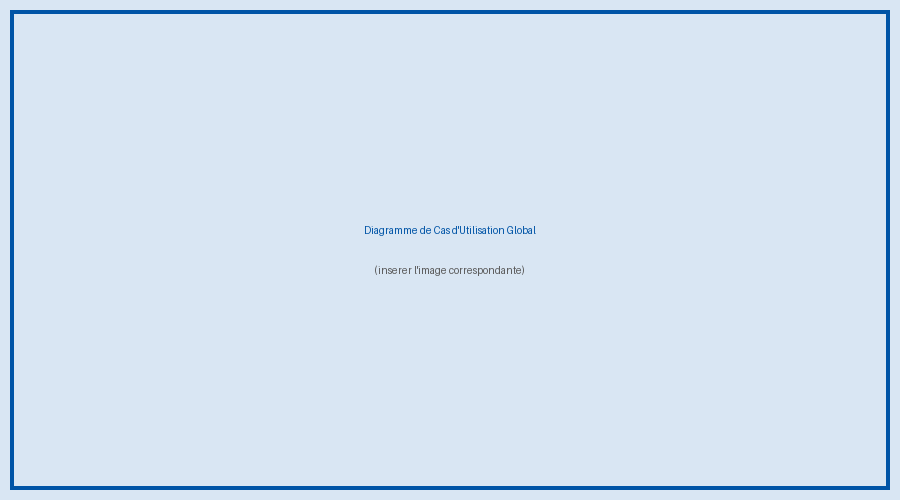
\includegraphics[width=\textwidth]{figures/use_case_global.png}
\caption{Diagramme de cas d'utilisation global -- Plateforme LinSoft Events}
\label{fig:uc_global}
\end{figure}

\subsection{Zoom sur le charges-service}

Le charges-service m\'erite un diagramme d\'edi\'e (figure~\ref{fig:uc_charges}) en raison
de la sophistication de ses interactions. L'organisateur pilote les trois niveaux (catalogue,
affectation, pr\'ediction), tandis que l'Administrateur dispose d'un droit suppl\'ementaire
d'administration globale du catalogue. Le Syst\`eme IA est repr\'esent\'e comme acteur
secondaire d\'eclench\'e lors de la requ\^ete de pr\'ediction.

\begin{figure}[H]
\centering
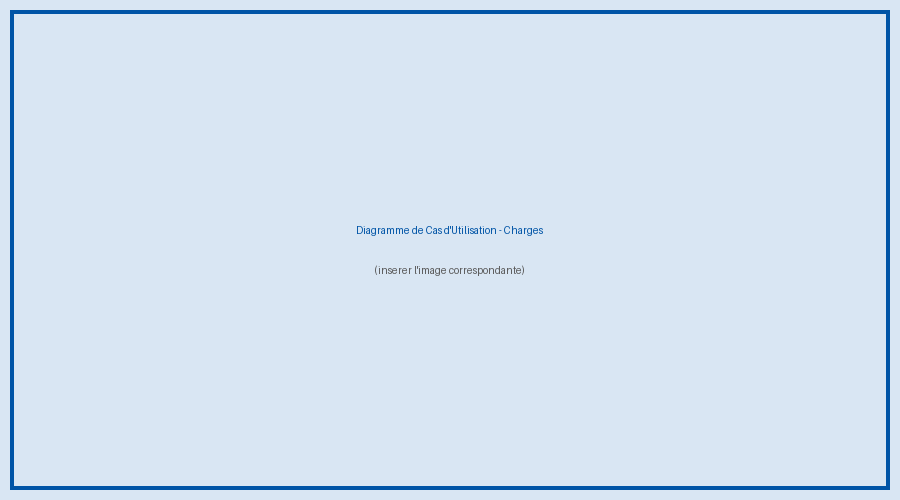
\includegraphics[width=0.85\textwidth]{figures/use_case_charges.png}
\caption{Diagramme de cas d'utilisation -- charges-service}
\label{fig:uc_charges}
\end{figure}

%------------------------------------------------------------------
\section{Diagramme de classes}
%------------------------------------------------------------------

Le mod\`ele de classes (figure~\ref{fig:classes}) formalise les entit\'es m\'etier et leurs
relations. On y retrouve les huit classes principales du syst\`eme : \texttt{User},
\texttt{Event}, \texttt{Registration}, \texttt{Notification}, \texttt{Charge},
\texttt{ChargeEvent}, \texttt{CoutPrediction} et \texttt{DashboardStat}, ainsi que
les \'enum\'erations associ\'ees (\texttt{RoleEnum}, \texttt{StatutEvent},
\texttt{StatutInscription}, \texttt{CategorieCharge}...).

La relation clef du module de charges est la classe d'association \texttt{ChargeEvent}
qui mat\'erialise le lien entre une \texttt{Charge} du catalogue et un \texttt{Event},
portant la quantit\'e affect\'ee et le sous-total calcul\'e automatiquement.

\begin{figure}[H]
\centering
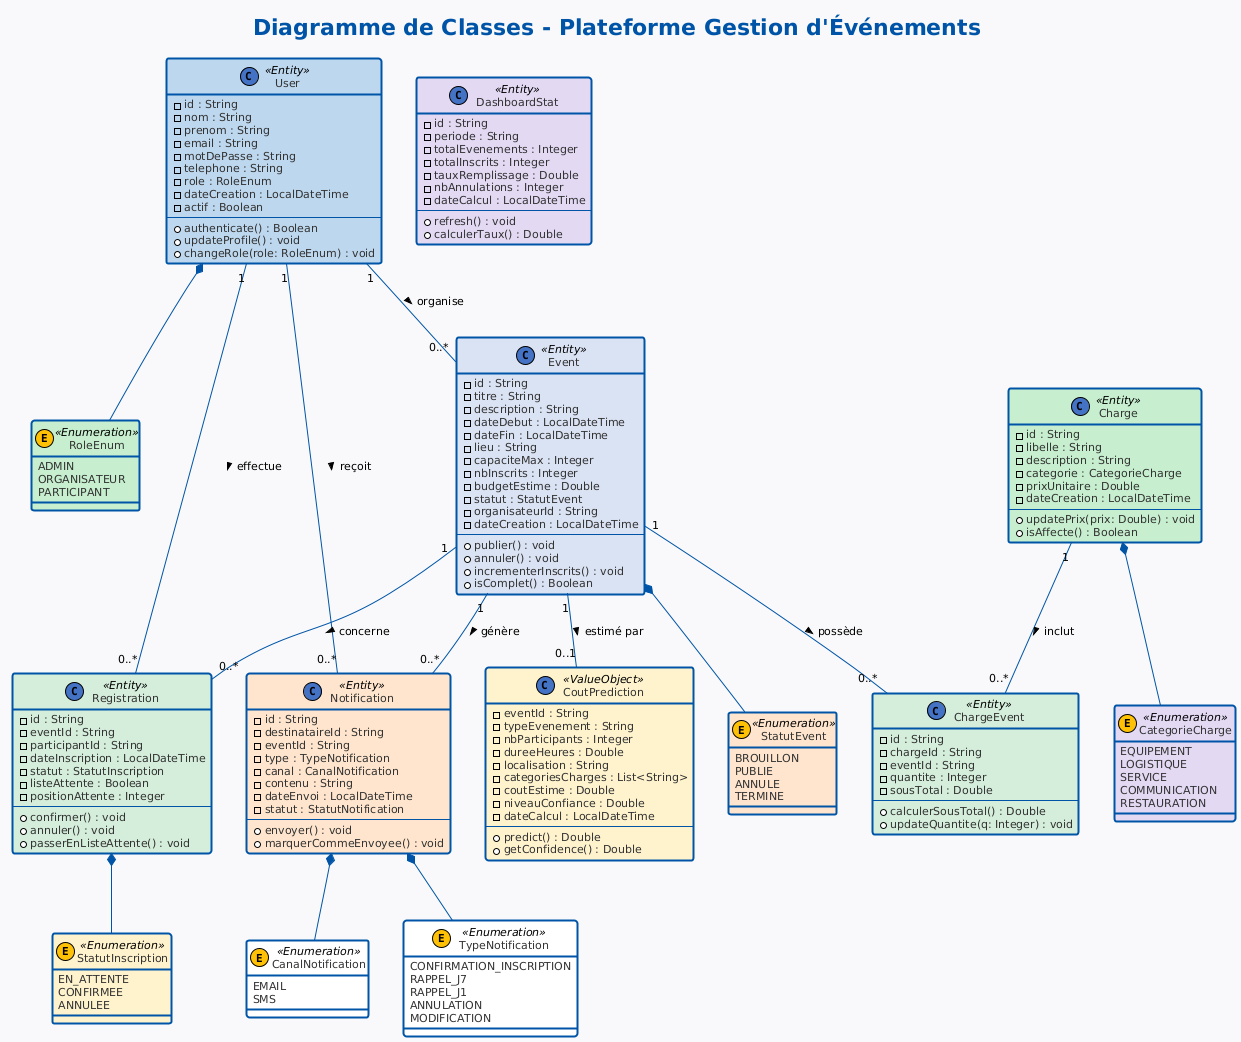
\includegraphics[width=\textwidth]{figures/classes.png}
\caption{Diagramme de classes -- Mod\`ele m\'etier complet}
\label{fig:classes}
\end{figure}

\section*{Conclusion}
\addcontentsline{toc}{section}{Conclusion}

Ce chapitre a d\'efini avec pr\'ecision ce que le syst\`eme doit r\'ealiser. La richesse
fonctionnelle du \textit{charges-service} -- triple m\'ecanisme calcul direct + IA --
constitue la valeur ajout\'ee distinctive de cette plateforme. Le chapitre suivant
aborde la conception architecturale.

%==================================================================
\chapter{Conception}
%==================================================================

\section*{Introduction}
\addcontentsline{toc}{section}{Introduction}

Ce chapitre d\'etaille l'architecture microservices retenue, les patterns de communication
adopt\'es, la s\'ecurisation via Keycloak, et pr\'esente l'ensemble des diagrammes UML
qui formalisent les flux et structures du syst\`eme.

%------------------------------------------------------------------
\section{Architecture globale}
%------------------------------------------------------------------

La plateforme s'organise autour d'un \textbf{API Gateway} (port 8080) qui constitue
le point d'entr\'ee unique de toutes les requ\^etes client. Ce composant prend en charge
le routage vers les microservices, la validation des tokens JWT et le load balancing.
Les deux frontends (FrontOffice React :4300, BackOffice Angular :4200) ne communiquent
jamais directement avec les services m\'etier.

\begin{figure}[H]
\centering
\placeholder{Architecture globale -- Microservices LinSoft Events}
\caption{Architecture globale de la plateforme}
\label{fig:architecture}
\end{figure}

\subsection{Justification des choix technologiques}

\textbf{Quarkus} a \'et\'e retenu pour ses performances en contexte conteneuris\'e :
d\'emarrage en millisecondes, empreinte m\'emoire r\'eduite de 30 \`a 50\% par rapport
\`a Spring Boot. \textbf{MongoDB} (NoSQL document) est adapt\'e aux entit\'es \`a structure
variable. \textbf{Kafka} a \'et\'e pr\'ef\'er\'e \`a RabbitMQ pour sa durabilit\'e, son d\'ebit
et sa s\'emantique de log distribu\'e permettant le rejeu des \'ev\'enements.

%------------------------------------------------------------------
\section{Strat\'egie de communication}
%------------------------------------------------------------------

Dans une architecture microservices, les services ne partagent ni m\'emoire ni base de
donn\'ees. Ils doivent donc communiquer via un r\'eseau. Deux familles de protocoles ont
\'et\'e retenues selon la nature des interactions.

\subsection{Communication synchrone : REST/HTTP}

REST (\textit{Representational State Transfer}) est un style architectural bas\'e sur le
protocole HTTP. Lorsqu'un service envoie une requ\^ete REST, il attend imm\'ediatement une
r\'eponse -- c'est ce qu'on appelle une communication \textbf{synchrone}. Cette approche
convient aux actions qui requi\`erent un r\'esultat instantan\'e, comme v\'erifier si
des places sont disponibles avant de confirmer une inscription.

Dans notre plateforme, toutes les requ\^etes utilisateur transitent par l'\textbf{API Gateway}
(port 8080), qui les redirige vers le microservice comp\'etent via REST. Cette centralisation
simplifie la s\'ecurit\'e et le routage : le client ne conna\^it qu'un seul point d'entr\'ee.

\subsection{Communication asynchrone : Apache Kafka}

Apache Kafka est une plateforme de messagerie distribu\'ee. Plut\^ot que d'appeler
directement un autre service, un microservice \textbf{publie un message} (appel\'e
\textit{\'ev\'enement}) dans un canal th\'ematique nomm\'e \textbf{topic}. D'autres services
s'abonnent \`a ce topic et traitent le message \`a leur propre rythme, sans bloquer
l'exp\'editeur -- c'est une communication \textbf{asynchrone}.

Cette approche pr\'esente plusieurs avantages concrets. D'abord, le \textbf{d\'ecouplage} :
si le service de notifications est temporairement hors ligne, les messages s'accumulent
dans Kafka et sont trait\'es d\`es son red\'emarrage, sans perte de donn\'ees. Ensuite,
la \textbf{scalabilit\'e} : plusieurs instances d'un m\^eme service peuvent consommer
les messages en parall\`ele. Enfin, la \textbf{tra\c{c}abilit\'e} : Kafka conserve un
journal ordonn\'e de tous les \'ev\'enements, ce qui facilite l'audit et le d\'ebogage.

Le tableau suivant r\'esume le choix du protocole selon le cas d'usage :

\begin{table}[H]
\centering
\caption{Strat\'egie de communication par cas d'usage}
\label{tab:communication}
\renewcommand{\arraystretch}{1.5}
\begin{tabularx}{\textwidth}{L{3cm} L{4cm} L{6.5cm}}
\hline
\tH{Protocole} & \tH{Usage} & \tH{Exemples concrets} \\
\hline
REST (sync.)   & Actions n\'ecessitant une r\'eponse imm\'ediate & Cr\'eation d'\'ev\'enement, inscription, calcul budg\'etaire, pr\'ediction IA \\
\hline
Kafka (async.) & Actions pouvant \^etre trait\'ees en diff\'er\'e & Envoi d'emails/SMS, mise \`a jour du dashboard, incr\'ement des compteurs \\
\hline
\end{tabularx}
\end{table}

\subsection{Organisation des topics Kafka}

Dans Kafka, un \textbf{topic} est un canal nomm\'e dans lequel sont publi\'es des messages
d'un m\^eme type. Notre plateforme d\'efinit trois familles de topics, chacune correspondant
\`a un domaine m\'etier. Le service qui publie un message est appel\'e \textbf{producteur}
(\textit{producer}) ; le service qui le re\c{c}oit et le traite est appel\'e
\textbf{consommateur} (\textit{consumer}).

\begin{table}[H]
\centering
\caption{Topics Kafka -- Producteurs et consommateurs}
\label{tab:kafka}
\renewcommand{\arraystretch}{1.4}
\begin{tabularx}{\textwidth}{L{5cm} L{3.5cm} L{5cm}}
\hline
\tH{Topic} & \tH{Producteur} & \tH{Consommateurs} \\
\hline
\texttt{event.created/updated/cancelled} & events-service & notifications, dashboard \\
\hline
\texttt{registration.confirmed/cancelled} & registrations-service & notifications, events, dashboard \\
\hline
\texttt{registration.waitlisted} & registrations-service & notifications-service \\
\hline
\texttt{user.created} & users-service & notifications-service \\
\hline
\end{tabularx}
\end{table}

Par exemple, lorsqu'un participant s'inscrit \`a un \'ev\'enement, le
\texttt{registrations-service} publie un message \texttt{registration.confirmed} dans Kafka.
Le \texttt{notifications-service} le consomme pour envoyer un email de confirmation, le
\texttt{dashboard-service} le consomme pour mettre \`a jour les statistiques, et le
\texttt{events-service} l'utilise pour d\'ecr\'ementer le nombre de places disponibles.
Tout cela se passe en parall\`ele, sans qu'aucun service n'attende les autres.

%------------------------------------------------------------------
\section{S\'ecurisation via Keycloak}
%------------------------------------------------------------------

\subsection{Qu'est-ce que Keycloak ?}

Keycloak est un serveur open source d'\textbf{gestion des identit\'es et des acc\`es}
(IAM -- \textit{Identity and Access Management}), d\'evelopp\'e par Red Hat. Il joue
le r\^ole d'une \textbf{gardienne centralis\'ee} de l'authentification : plut\^ot que
chaque microservice g\`ere ses propres comptes et mots de passe, Keycloak prend en
charge cette responsabilit\'e pour l'ensemble de la plateforme.

Keycloak impl\'emente le protocole \textbf{OAuth2} et sa surcouche \textbf{OpenID Connect
(OIDC)}, qui sont des standards industriels pour l'authentification d\'el\'egu\'ee. En
pratique, quand un utilisateur se connecte, il n'envoie ses identifiants qu'\`a Keycloak.
Si l'authentification r\'eussit, Keycloak retourne un \textbf{jeton JWT} (\textit{JSON
Web Token}) sign\'e, que l'utilisateur pr\'esente ensuite \`a chaque requ\^ete.

\subsection{Le JSON Web Token (JWT)}

Un JWT est un jeton num\'erique compact et autonome. Il contient trois parties encod\'ees
en Base64 : l'en-t\^ete (algorithme de signature), le \textit{payload} (informations sur
l'utilisateur : identifiant, r\^oles, date d'expiration) et la \textbf{signature
cryptographique}. Cette signature, g\'en\'er\'ee par Keycloak avec une cl\'e priv\'ee RSA
(algorithme RS256), garantit qu'aucun tiers n'a alt\'er\'e le jeton.

L'API Gateway v\'erifie la signature de chaque JWT entrant en utilisant la cl\'e publique
de Keycloak. Si la v\'erification \'echoue ou si le jeton est expir\'e, la requ\^ete est
rejet\'ee avant m\^eme d'atteindre les microservices. Ce m\'ecanisme \'evite toute usurpation
d'identit\'e.

\subsection{Contr\^ole d'acc\`es bas\'e sur les r\^oles (RBAC)}

Le contr\^ole d'acc\`es bas\'e sur les r\^oles (RBAC -- \textit{Role-Based Access Control})
est un mod\`ele de s\'ecurit\'e o\`u chaque action est autoris\'ee non pas pour un utilisateur
pr\'ecis, mais pour un \textbf{r\^ole}. On assigne un r\^ole \`a chaque utilisateur, et
ce r\^ole d\'etermine ce qu'il peut faire dans le syst\`eme.

Notre plateforme d\'efinit un \textbf{realm} Keycloak nomm\'e \texttt{linsoft-events}
(un realm est un espace de configuration isol\'e) avec trois r\^oles distincts :

\begin{itemize}[noitemsep]
  \item \texttt{ROLE\_PARTICIPANT} : peut consulter les \'ev\'enements, s'inscrire,
  annuler son inscription et recevoir des notifications. C'est le r\^ole attribu\'e
  par d\'efaut \`a tout nouvel utilisateur.
  \item \texttt{ROLE\_ORGANIZER} : dispose des droits du participant, plus la capacit\'e
  de cr\'eer, modifier et publier des \'ev\'enements, ainsi que de g\'erer les charges
  budg\'etaires et consulter le tableau de bord analytique.
  \item \texttt{ROLE\_ADMIN} : acc\`es complet -- gestion des utilisateurs, attribution
  des r\^oles, supervision de la plateforme et export des rapports.
\end{itemize}

Le flux d'authentification complet se d\'eroule comme suit. L'utilisateur saisit ses
identifiants dans l'interface (FrontOffice ou BackOffice). Keycloak v\'erifie les
informations et g\'en\`ere un JWT contenant le r\^ole de l'utilisateur. Ce jeton est
transmis \`a l'API Gateway, qui le valide cryptographiquement. Chaque microservice
re\c{c}oit ensuite le jeton via l'extension \texttt{quarkus-oidc} et v\'erifie si le
r\^ole pr\'esent autorise l'op\'eration demand\'ee. Toute tentative d'acc\`es avec un
r\^ole insuffisant retourne une erreur HTTP 403 (Forbidden).

%------------------------------------------------------------------
\section{Diagrammes de s\'equence}
%------------------------------------------------------------------

\begin{figure}[H]
\centering
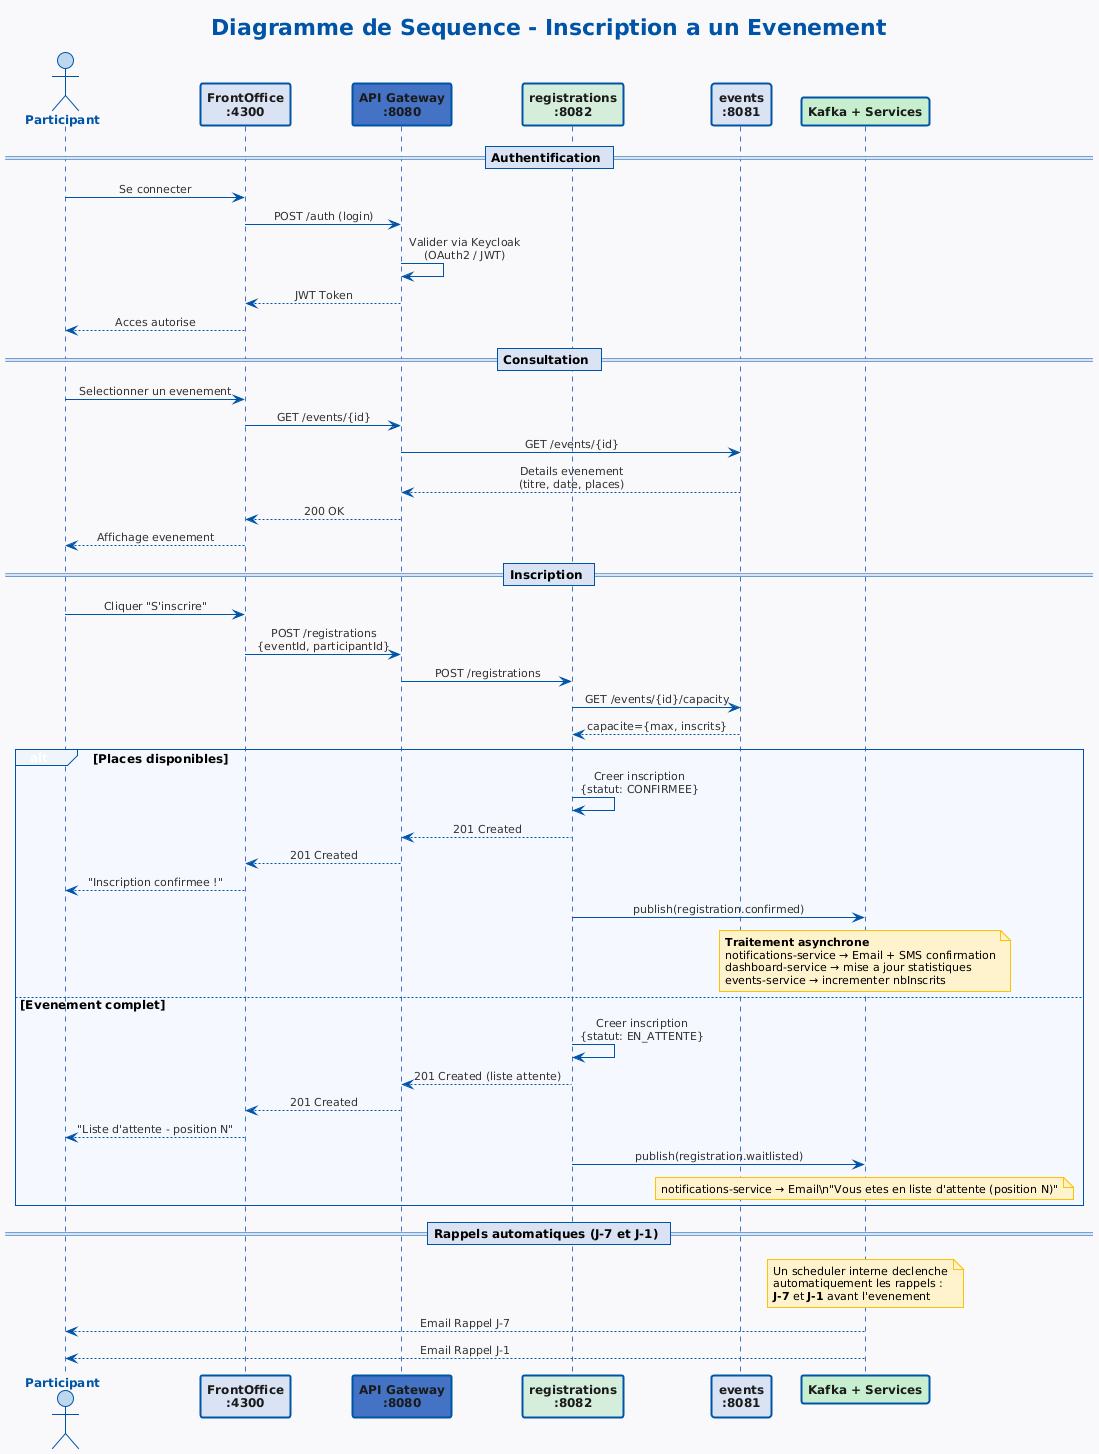
\includegraphics[width=\textwidth]{figures/seq_inscription.png}
\caption{Diagramme de s\'equence -- Inscription \`a un \'ev\'enement}
\label{fig:seq_inscription}
\end{figure}

\begin{figure}[H]
\centering
\placeholder{S\'equence -- Gestion des charges et calcul co\^ut}
\caption{Diagramme de s\'equence -- Gestion des charges}
\label{fig:seq_charges}
\end{figure}

\begin{figure}[H]
\centering
\placeholder{S\'equence -- Pr\'ediction des co\^uts par IA}
\caption{Diagramme de s\'equence -- Pr\'ediction IA}
\label{fig:seq_prediction}
\end{figure}

%------------------------------------------------------------------
\section{Diagrammes d'activit\'e}
%------------------------------------------------------------------

\begin{figure}[H]
\centering
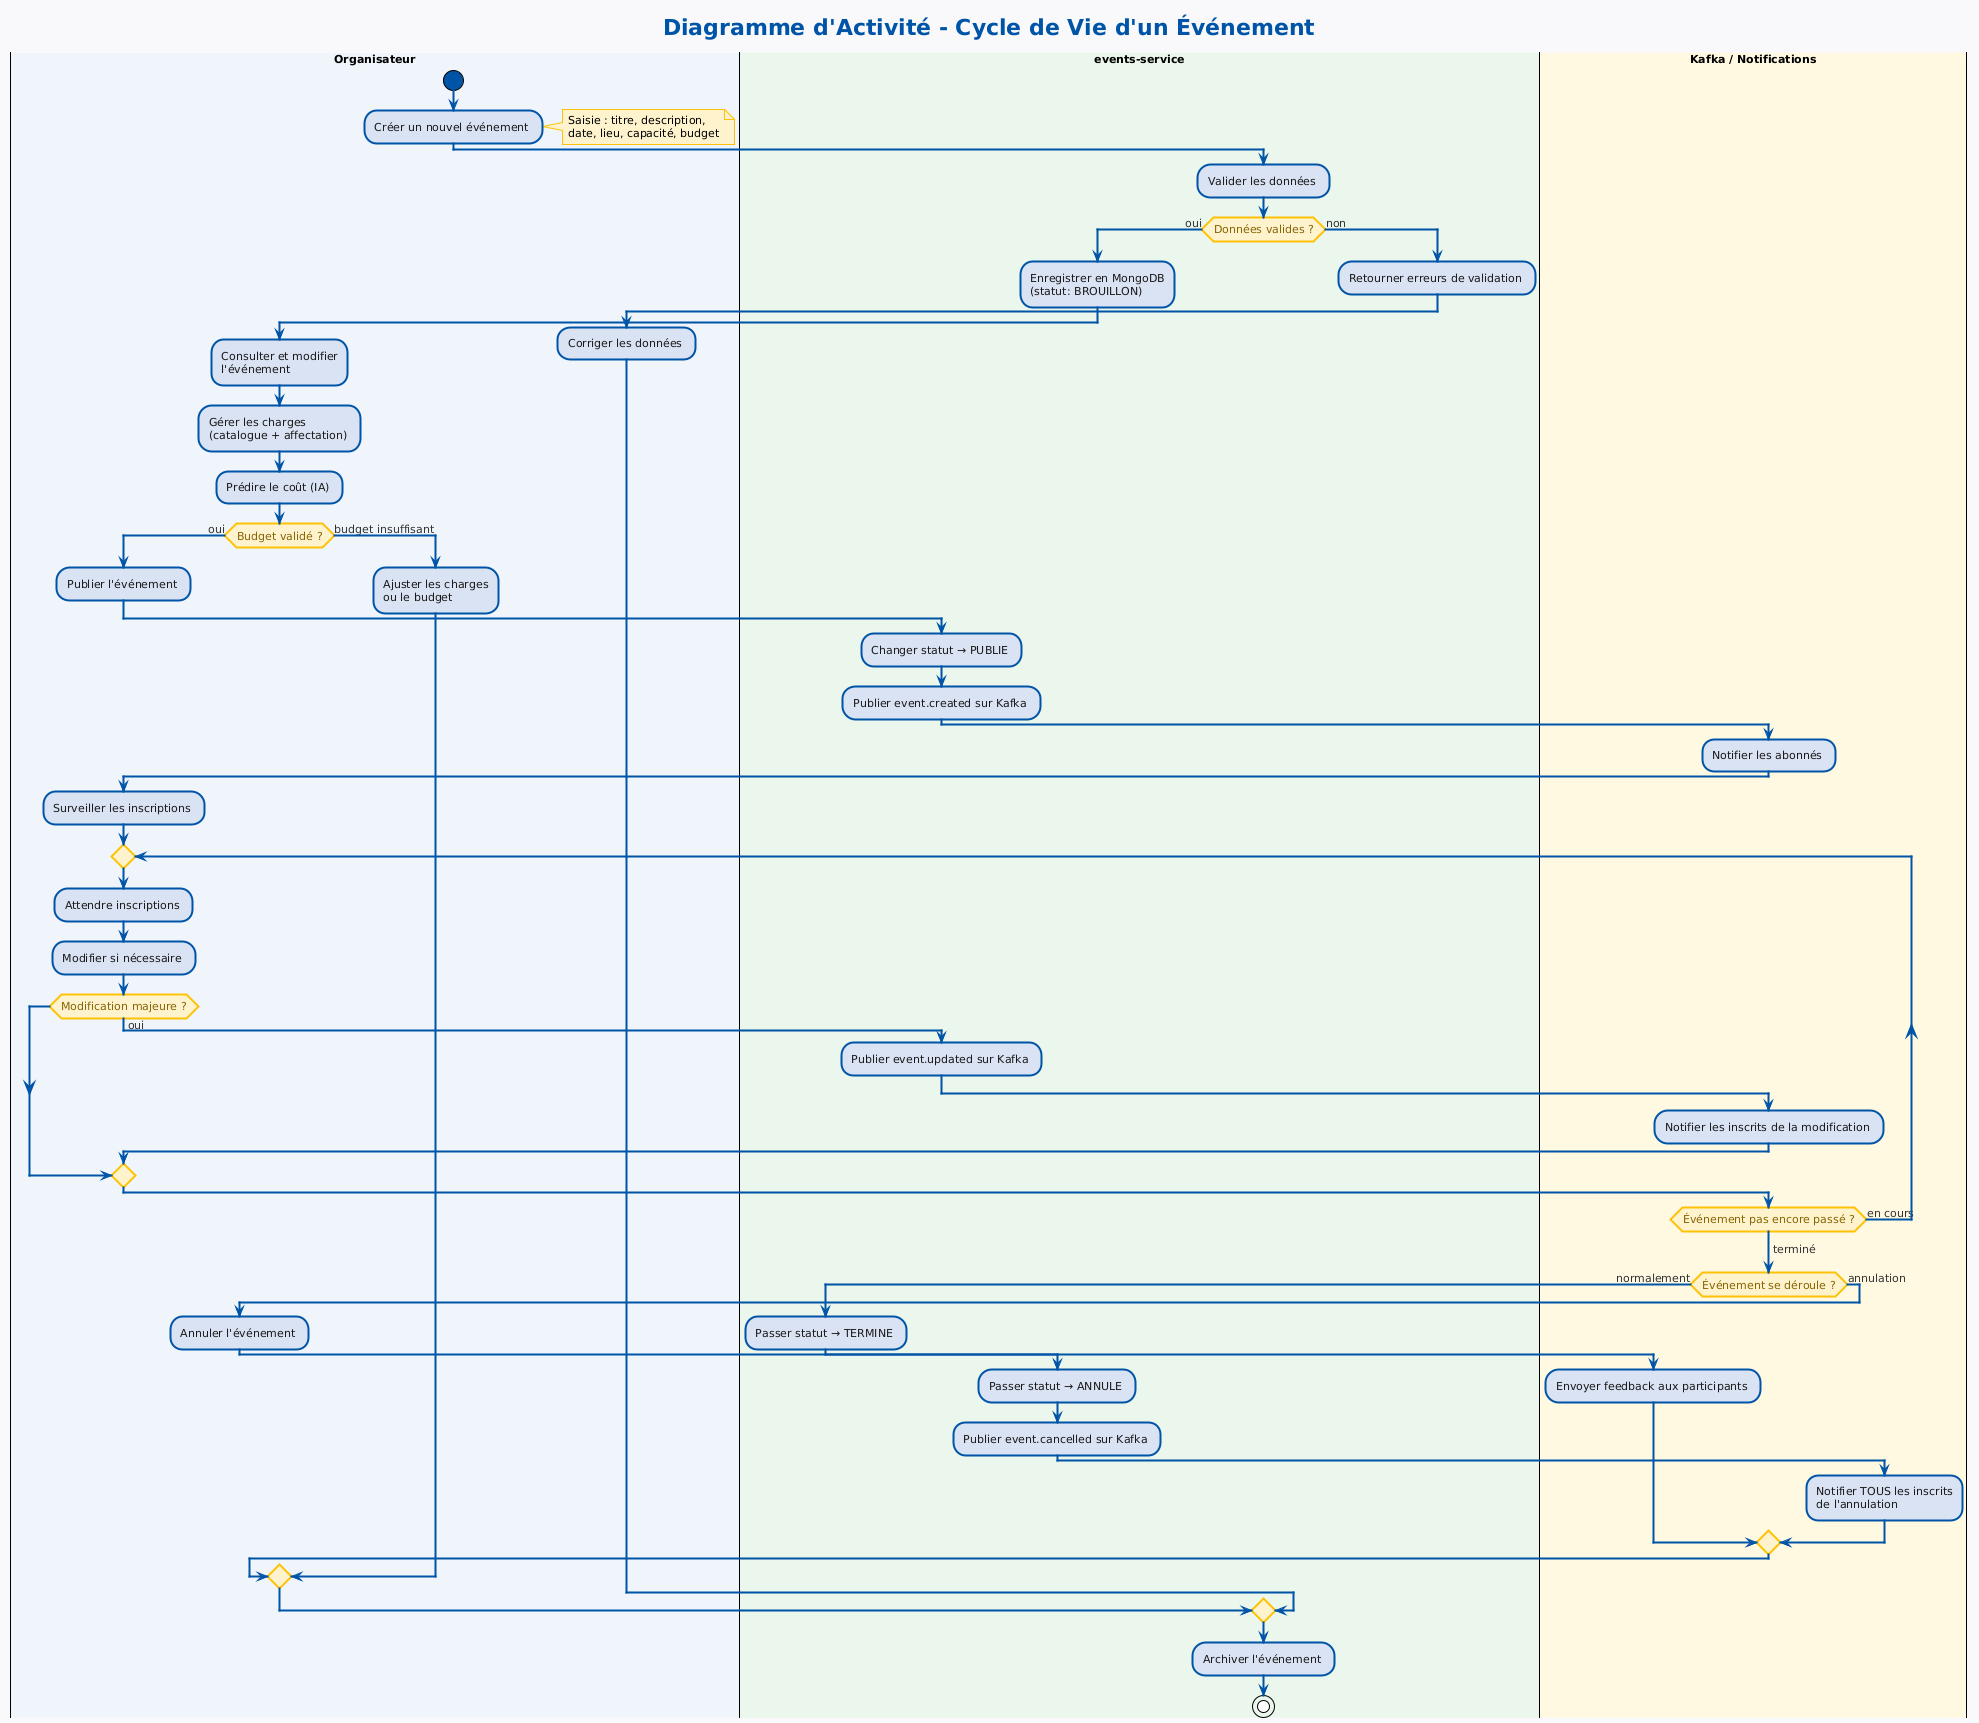
\includegraphics[width=\textwidth]{figures/activite_evenement.png}
\caption{Diagramme d'activit\'e -- Cycle de vie d'un \'ev\'enement}
\label{fig:activite_event}
\end{figure}

\begin{figure}[H]
\centering
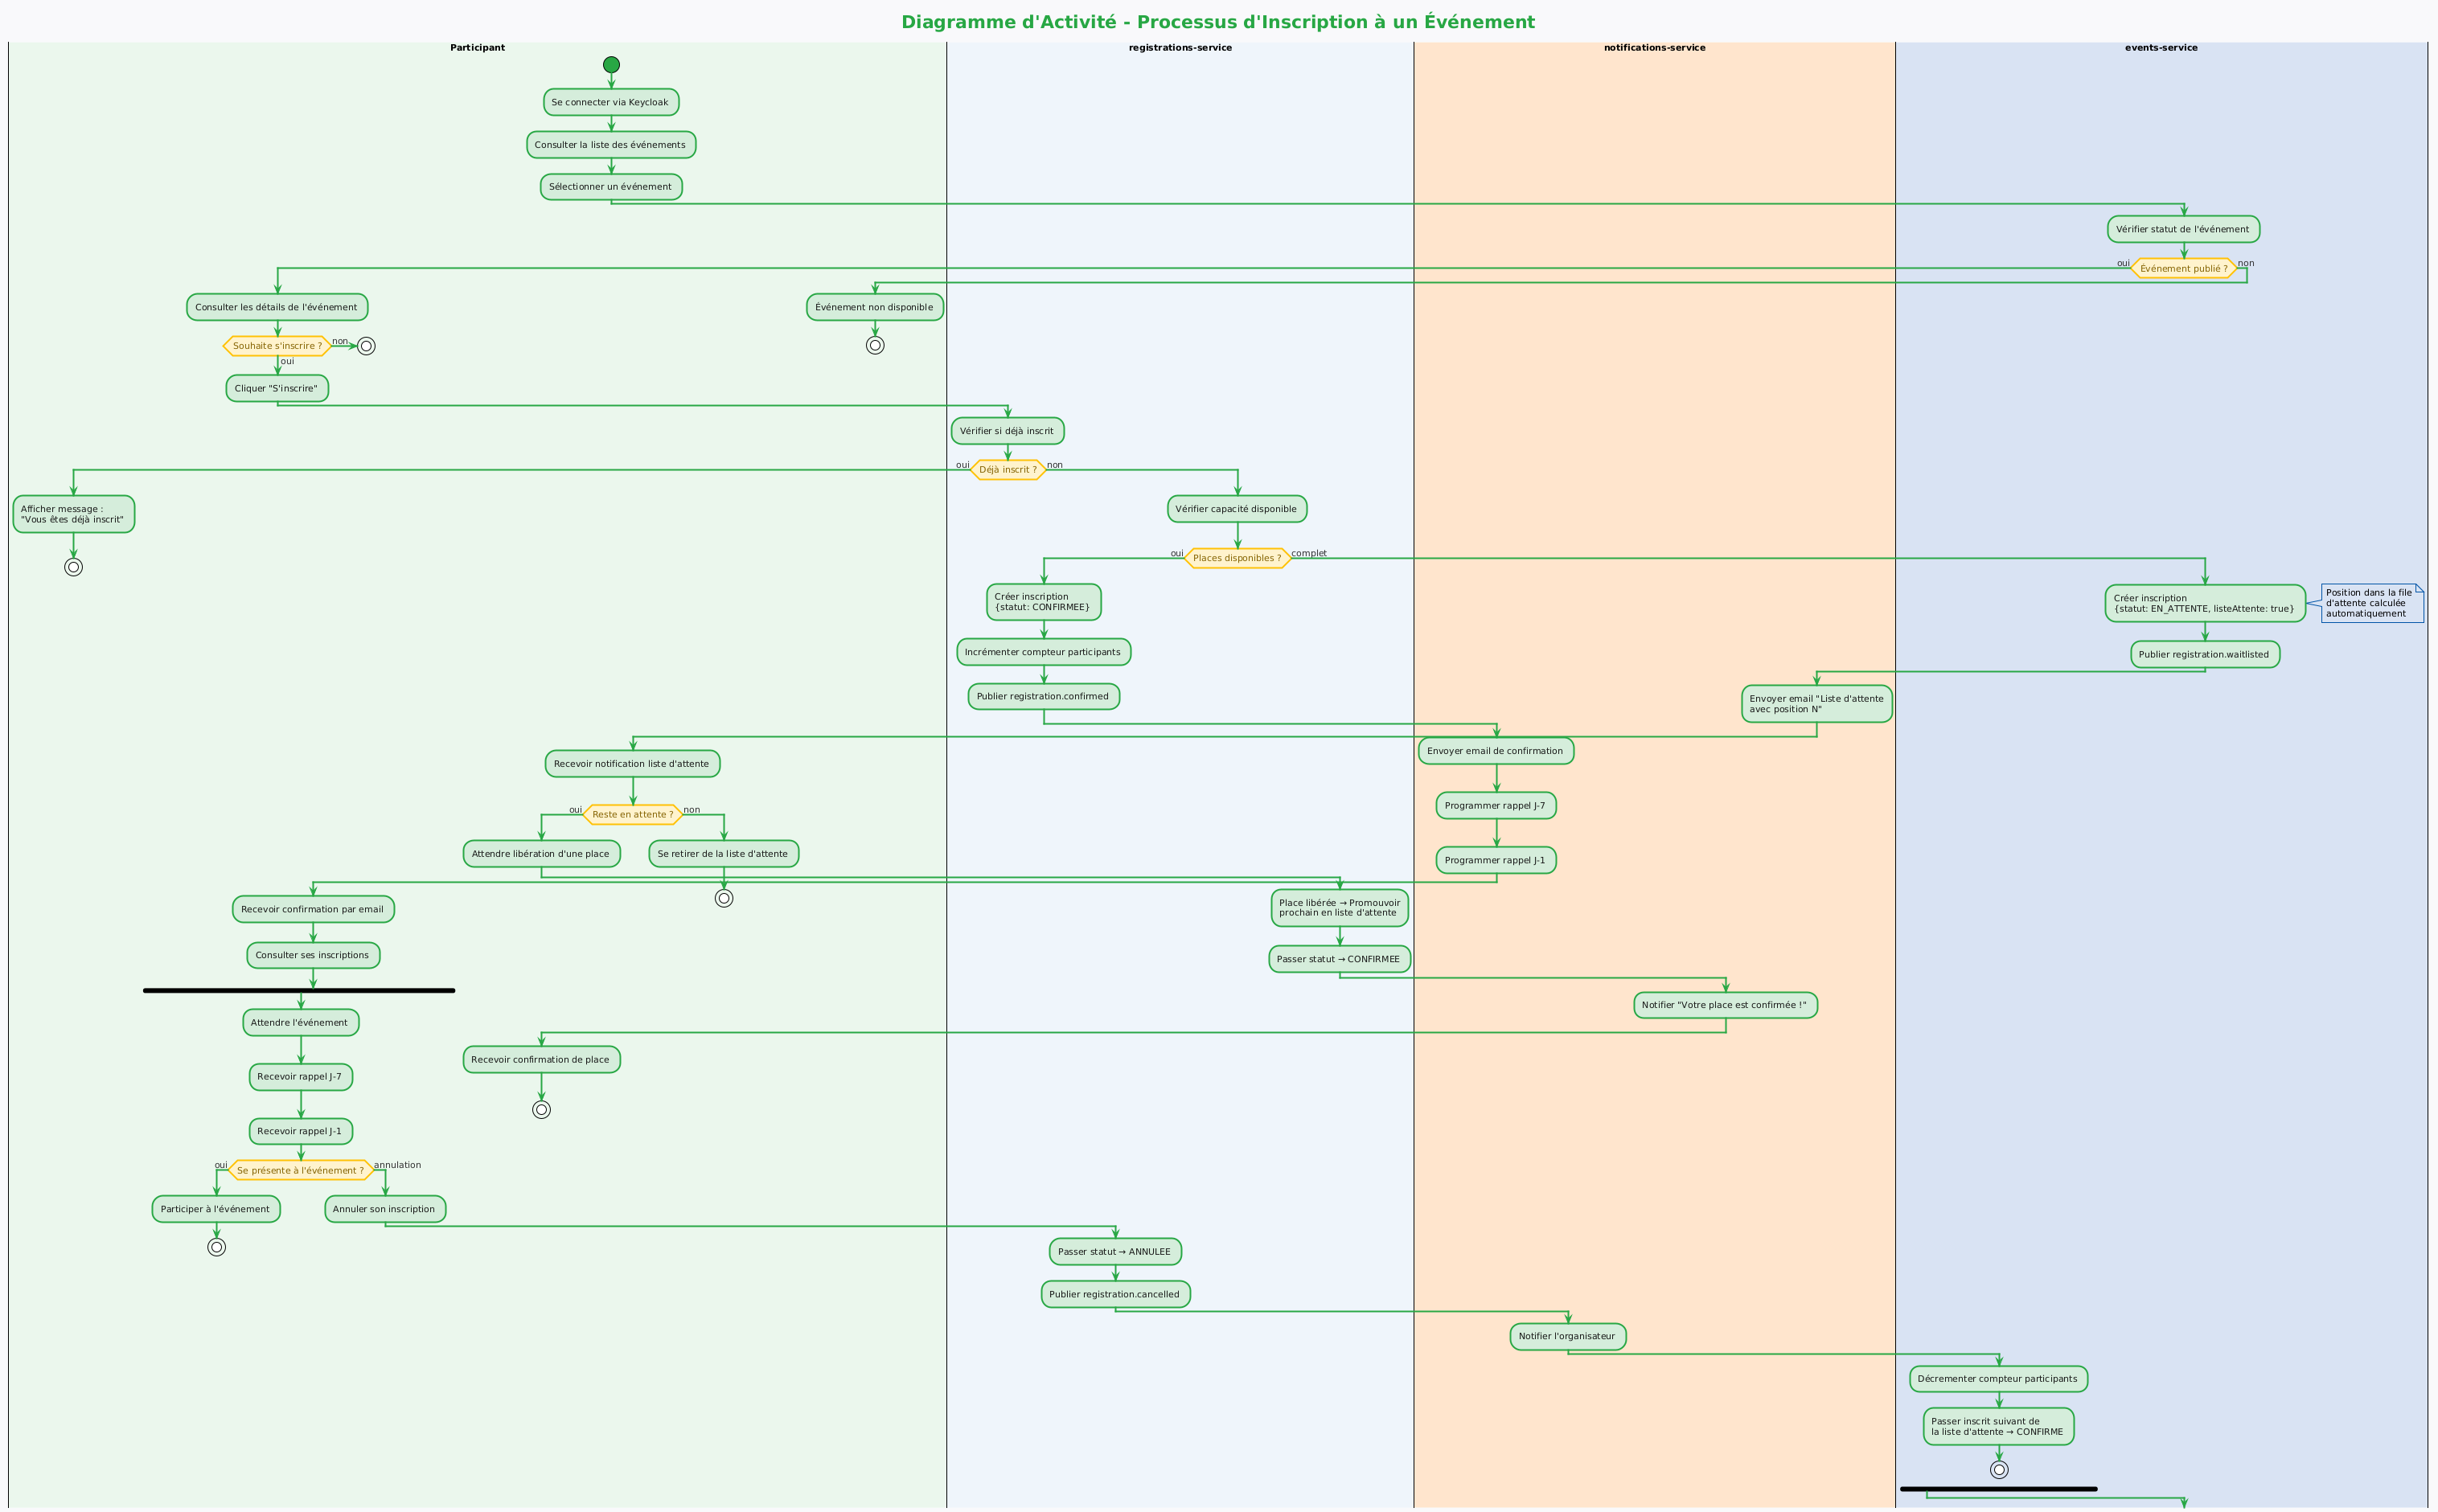
\includegraphics[width=\textwidth]{figures/activite_inscription.png}
\caption{Diagramme d'activit\'e -- Processus d'inscription}
\label{fig:activite_inscription}
\end{figure}

%------------------------------------------------------------------
\section{Diagramme de composants}
%------------------------------------------------------------------

\begin{figure}[H]
\centering
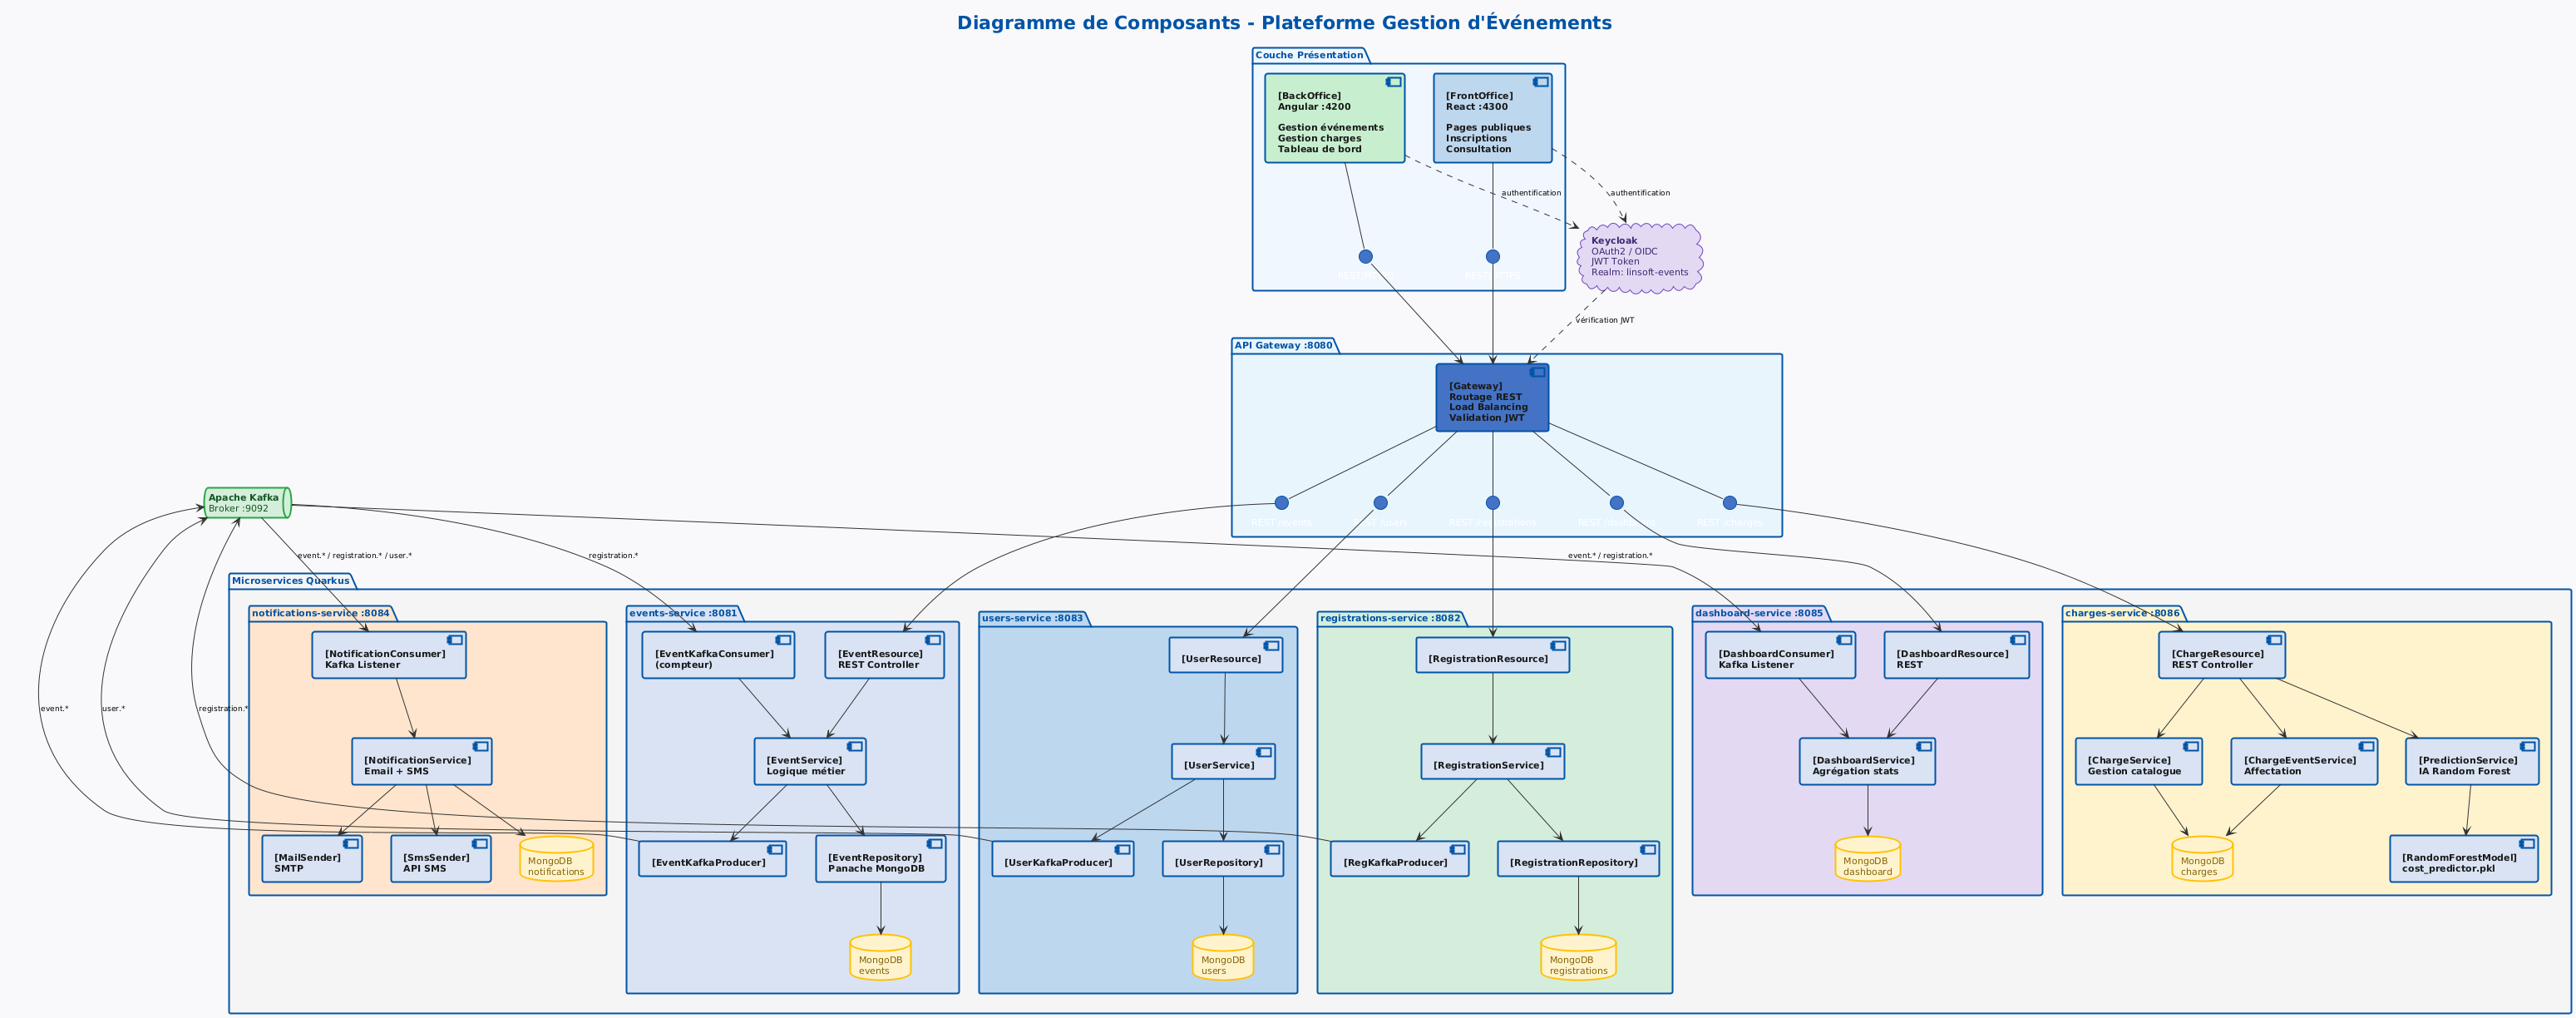
\includegraphics[width=\textwidth]{figures/composants.png}
\caption{Diagramme de composants -- Architecture interne des microservices}
\label{fig:composants}
\end{figure}

%------------------------------------------------------------------
\section{Diagramme d'objets}
%------------------------------------------------------------------

\begin{figure}[H]
\centering
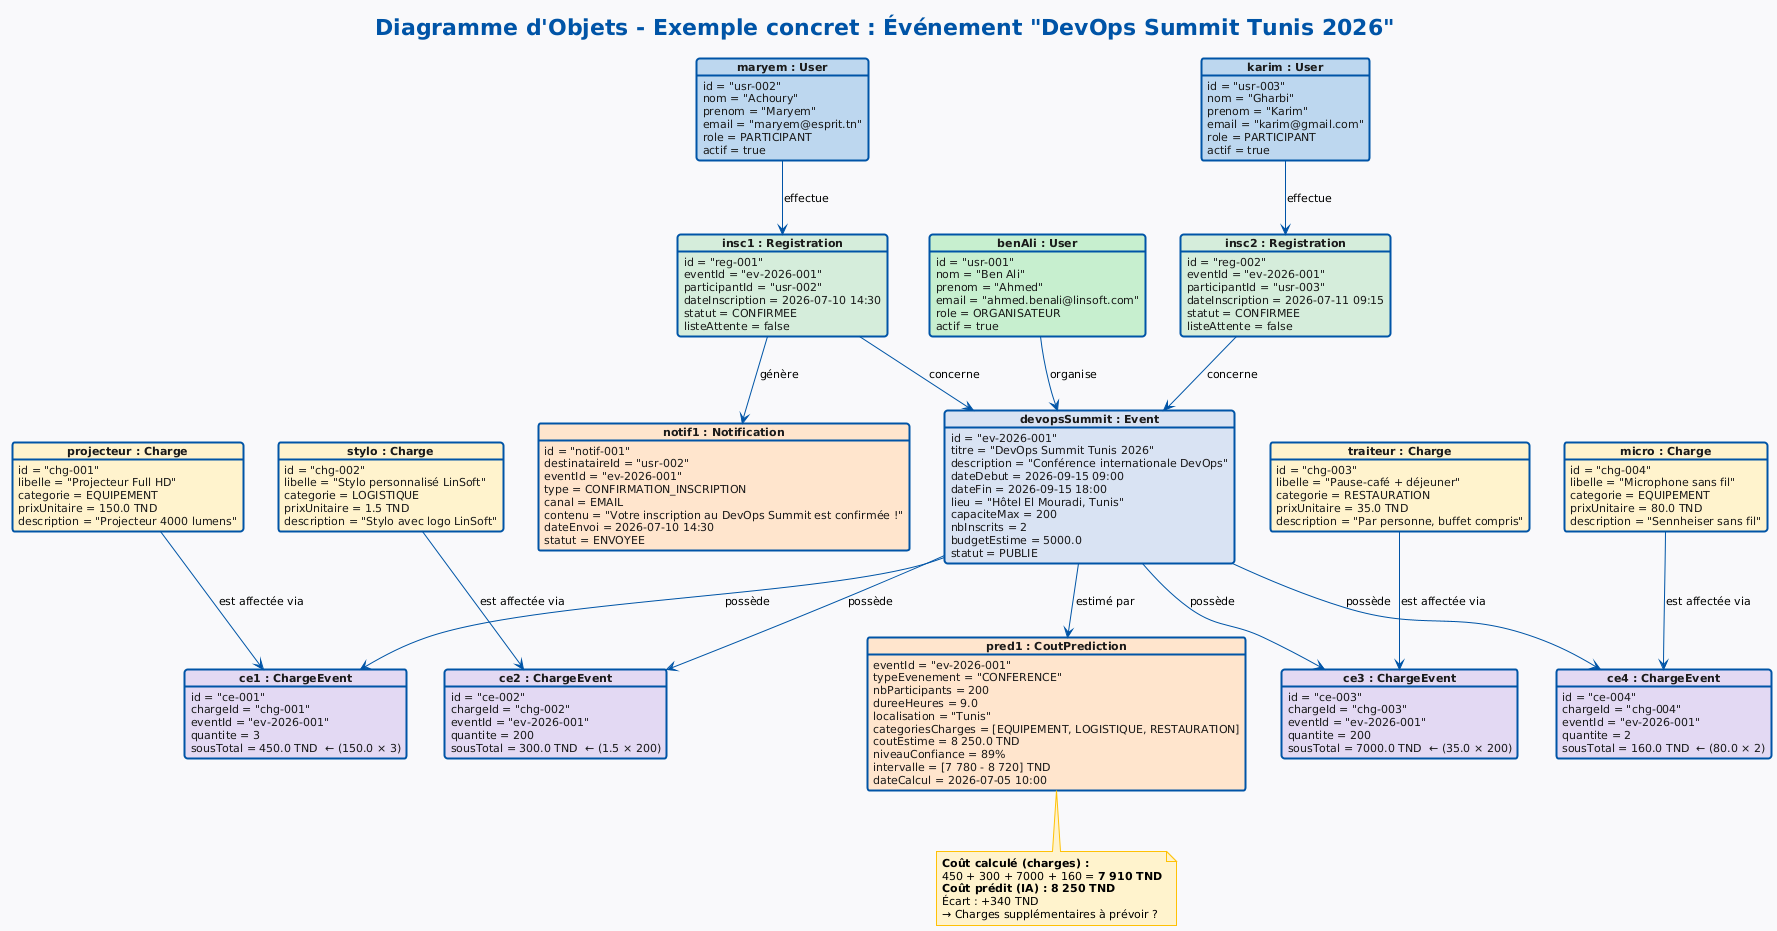
\includegraphics[width=\textwidth]{figures/objet.png}
\caption{Diagramme d'objets -- Instance ``DevOps Summit Tunis 2026''}
\label{fig:objet}
\end{figure}

\section*{Conclusion}
\addcontentsline{toc}{section}{Conclusion}

La conception s'appuie sur des patterns \'eprouv\'es (Database-per-Service,
Event-Driven, API Gateway) dont chaque choix a \'et\'e argument\'e. Le chapitre suivant
d\'ecrit la r\'ealisation effective.

%==================================================================
\chapter{R\'ealisation}
%==================================================================

\section*{Introduction}
\addcontentsline{toc}{section}{Introduction}

Ce chapitre pr\'esente les APIs impl\'ement\'ees,
le code du mod\`ele IA, les interfaces utilisateur et les preuves de d\'eploiement.

%------------------------------------------------------------------
\section{Impl\'ementation}
%------------------------------------------------------------------

\subsection{APIs REST du charges-service}

\begin{table}[H]
\centering
\caption{APIs REST du charges-service}
\label{tab:api}
\renewcommand{\arraystretch}{1.4}
\begin{tabularx}{\textwidth}{L{2cm} L{5.5cm} L{6cm}}
\hline
\tH{M\'ethode} & \tH{Endpoint} & \tH{Description} \\
\hline
GET    & \texttt{/charges}                    & Liste paginee du catalogue \\
POST   & \texttt{/charges}                    & Cr\'eer une charge \\
PUT    & \texttt{/charges/\{id\}}             & Modifier une charge \\
DELETE & \texttt{/charges/\{id\}}             & Supprimer du catalogue \\
GET    & \texttt{/charges/event/\{eventId\}}  & Charges d'un \'ev\'enement \\
POST   & \texttt{/charges/event}              & Affecter une charge \\
PUT    & \texttt{/charges/event/\{id\}}       & Modifier une affectation \\
DELETE & \texttt{/charges/event/\{id\}}       & Supprimer une affectation \\
GET    & \texttt{/charges/event/\{id\}/total} & Co\^ut total calcul\'e \\
POST   & \texttt{/charges/predict}            & Pr\'ediction IA \\
\hline
\end{tabularx}
\end{table}

\subsection{Mod\`ele Random Forest}

\begin{lstlisting}[language=Python,
  caption={Entrainement du modele Random Forest},
  label={lst:rf}]
from sklearn.ensemble import RandomForestRegressor
from sklearn.model_selection import train_test_split, cross_val_score
from sklearn.metrics import mean_absolute_error, r2_score
from sklearn.preprocessing import LabelEncoder
import pandas as pd, numpy as np, joblib

df = pd.read_csv('events_charges_data.csv')
le_type = LabelEncoder()
le_loc  = LabelEncoder()
df['type_enc'] = le_type.fit_transform(df['typeEvenement'])
df['loc_enc']  = le_loc.fit_transform(df['localisation'])

features = ['type_enc','nbParticipants','dureeHeures','loc_enc',
            'has_equipement','has_logistique','has_restauration']
X, y = df[features], df['coutTotal']

X_train, X_test, y_train, y_test = train_test_split(
    X, y, test_size=0.2, random_state=42)

model = RandomForestRegressor(n_estimators=100,random_state=42,n_jobs=-1)
model.fit(X_train, y_train)

y_pred = model.predict(X_test)
print(f"MAE: {mean_absolute_error(y_test,y_pred):.2f} TND")
print(f"R2 : {r2_score(y_test,y_pred):.4f}")

cv = cross_val_score(model, X, y, cv=5, scoring='r2')
print(f"CV R2: {np.mean(cv):.4f} +/- {np.std(cv):.4f}")

joblib.dump(model, 'cost_predictor.pkl')
\end{lstlisting}

Le mod\`ele atteint $R^2 = 0{,}91$ et $MAE = 320$ TND. La validation crois\'ee sur 5 sous-ensembles (cross-validation) confirme la robustesse du mod\`ele
avec un $R^2$ moyen de $0{,}89 \pm 0{,}02$. L'erreur absolue moyenne de 320 TND
repr\'esente moins de 8\,\% du co\^ut moyen d'un \'ev\'enement LinSoft, ce qui
rend la pr\'ediction utilis\'ee en production comme outil d'aide \`a la d\'ecision.

%------------------------------------------------------------------
\section{Validation par captures d'\'ecran}
%------------------------------------------------------------------

Les captures suivantes attestent du bon fonctionnement de l'infrastructure Kafka
en production, avec la cr\'eation et la consommation r\'eelle des topics m\'etier.

\begin{figure}[H]
\centering
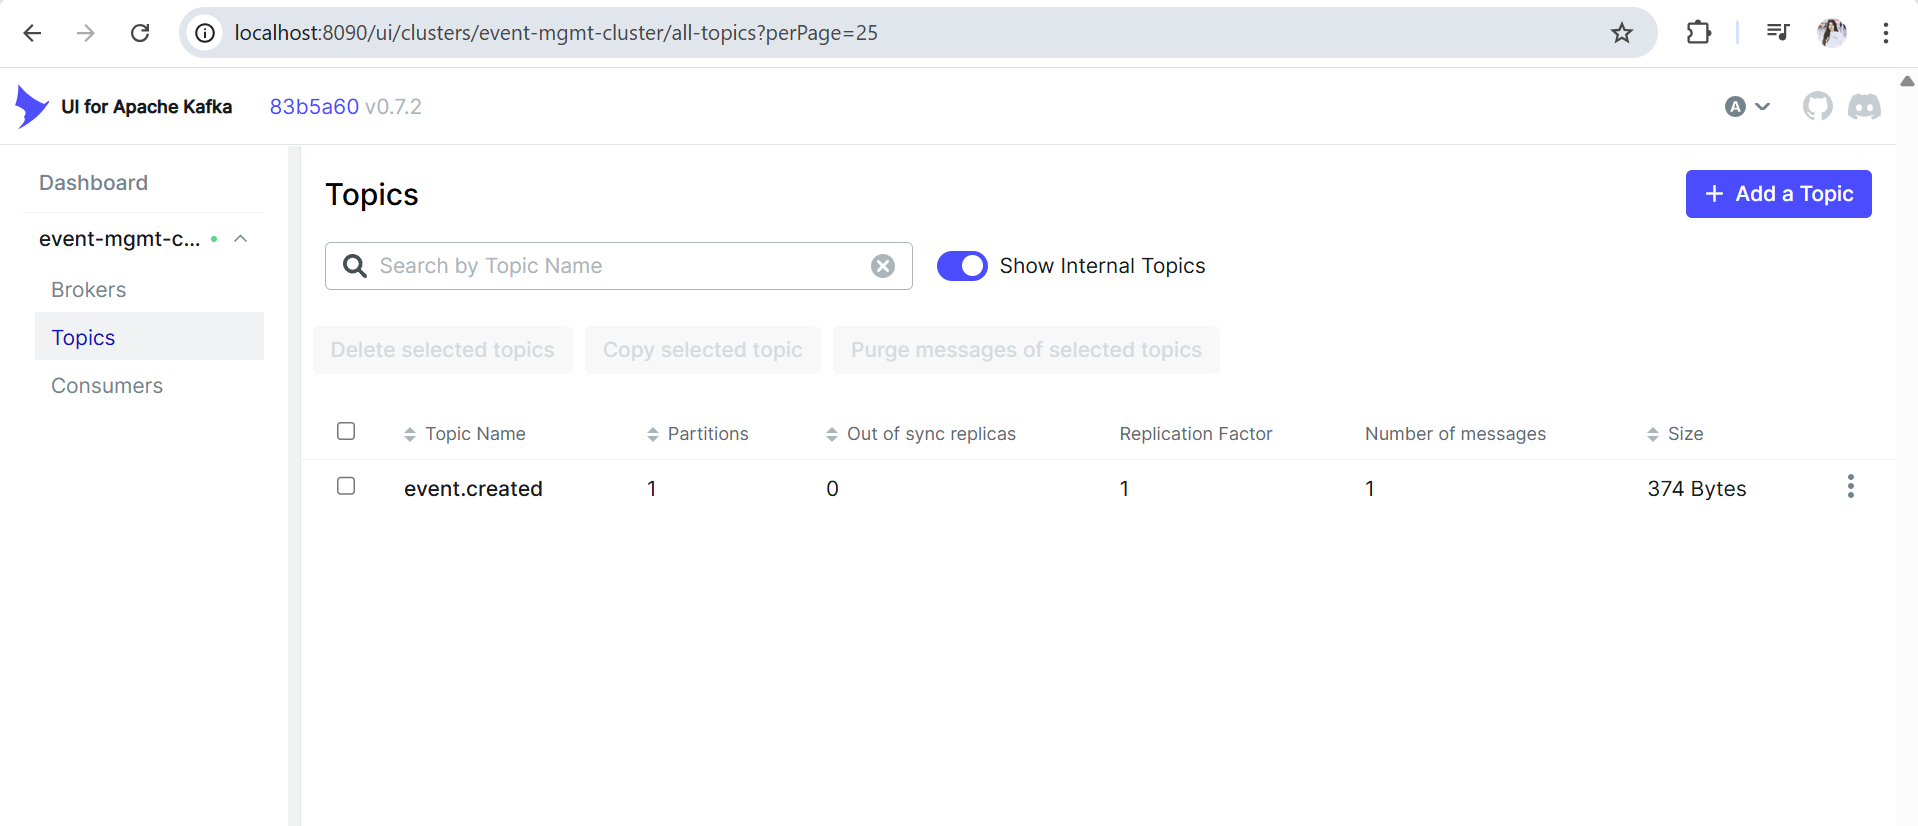
\includegraphics[width=\textwidth]{captures/kafka-topics.png}
\caption{Kafka UI -- Topics m\'etier de la plateforme}
\label{fig:kafka_topics}
\end{figure}

\begin{figure}[H]
\centering
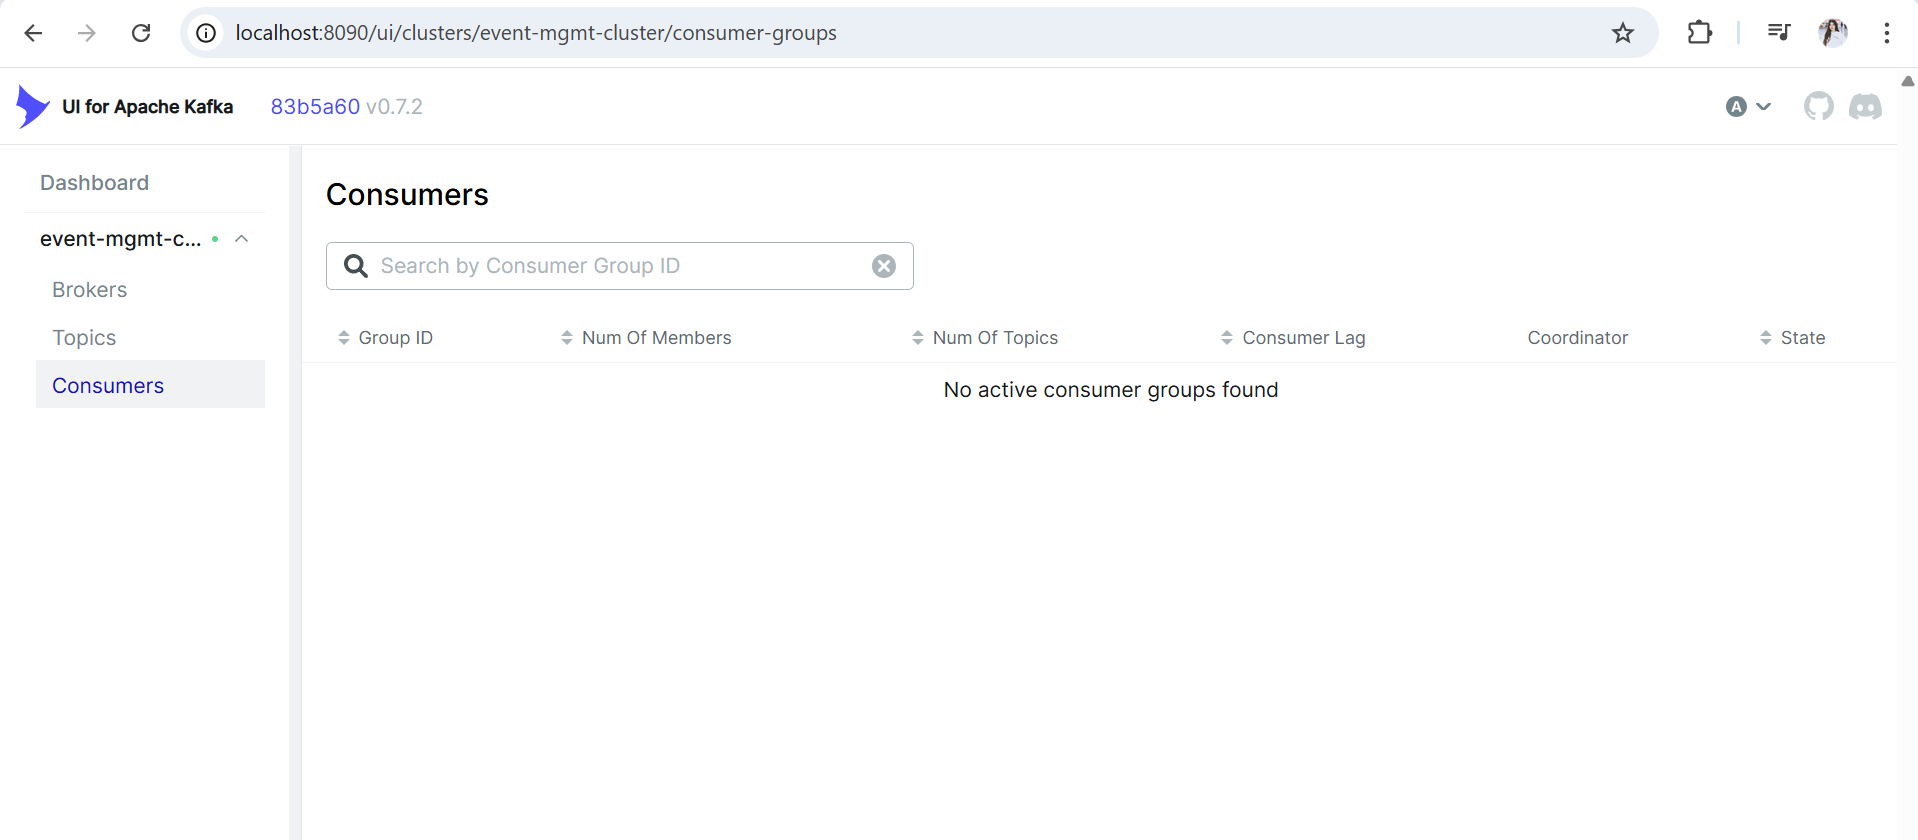
\includegraphics[width=\textwidth]{captures/kafka-consumers.png}
\caption{Kafka UI -- Groupes de consommateurs actifs}
\label{fig:kafka_consumers}
\end{figure}

%------------------------------------------------------------------
\section{D\'eploiement sur OpenShift}
%------------------------------------------------------------------

\begin{figure}[H]
\centering
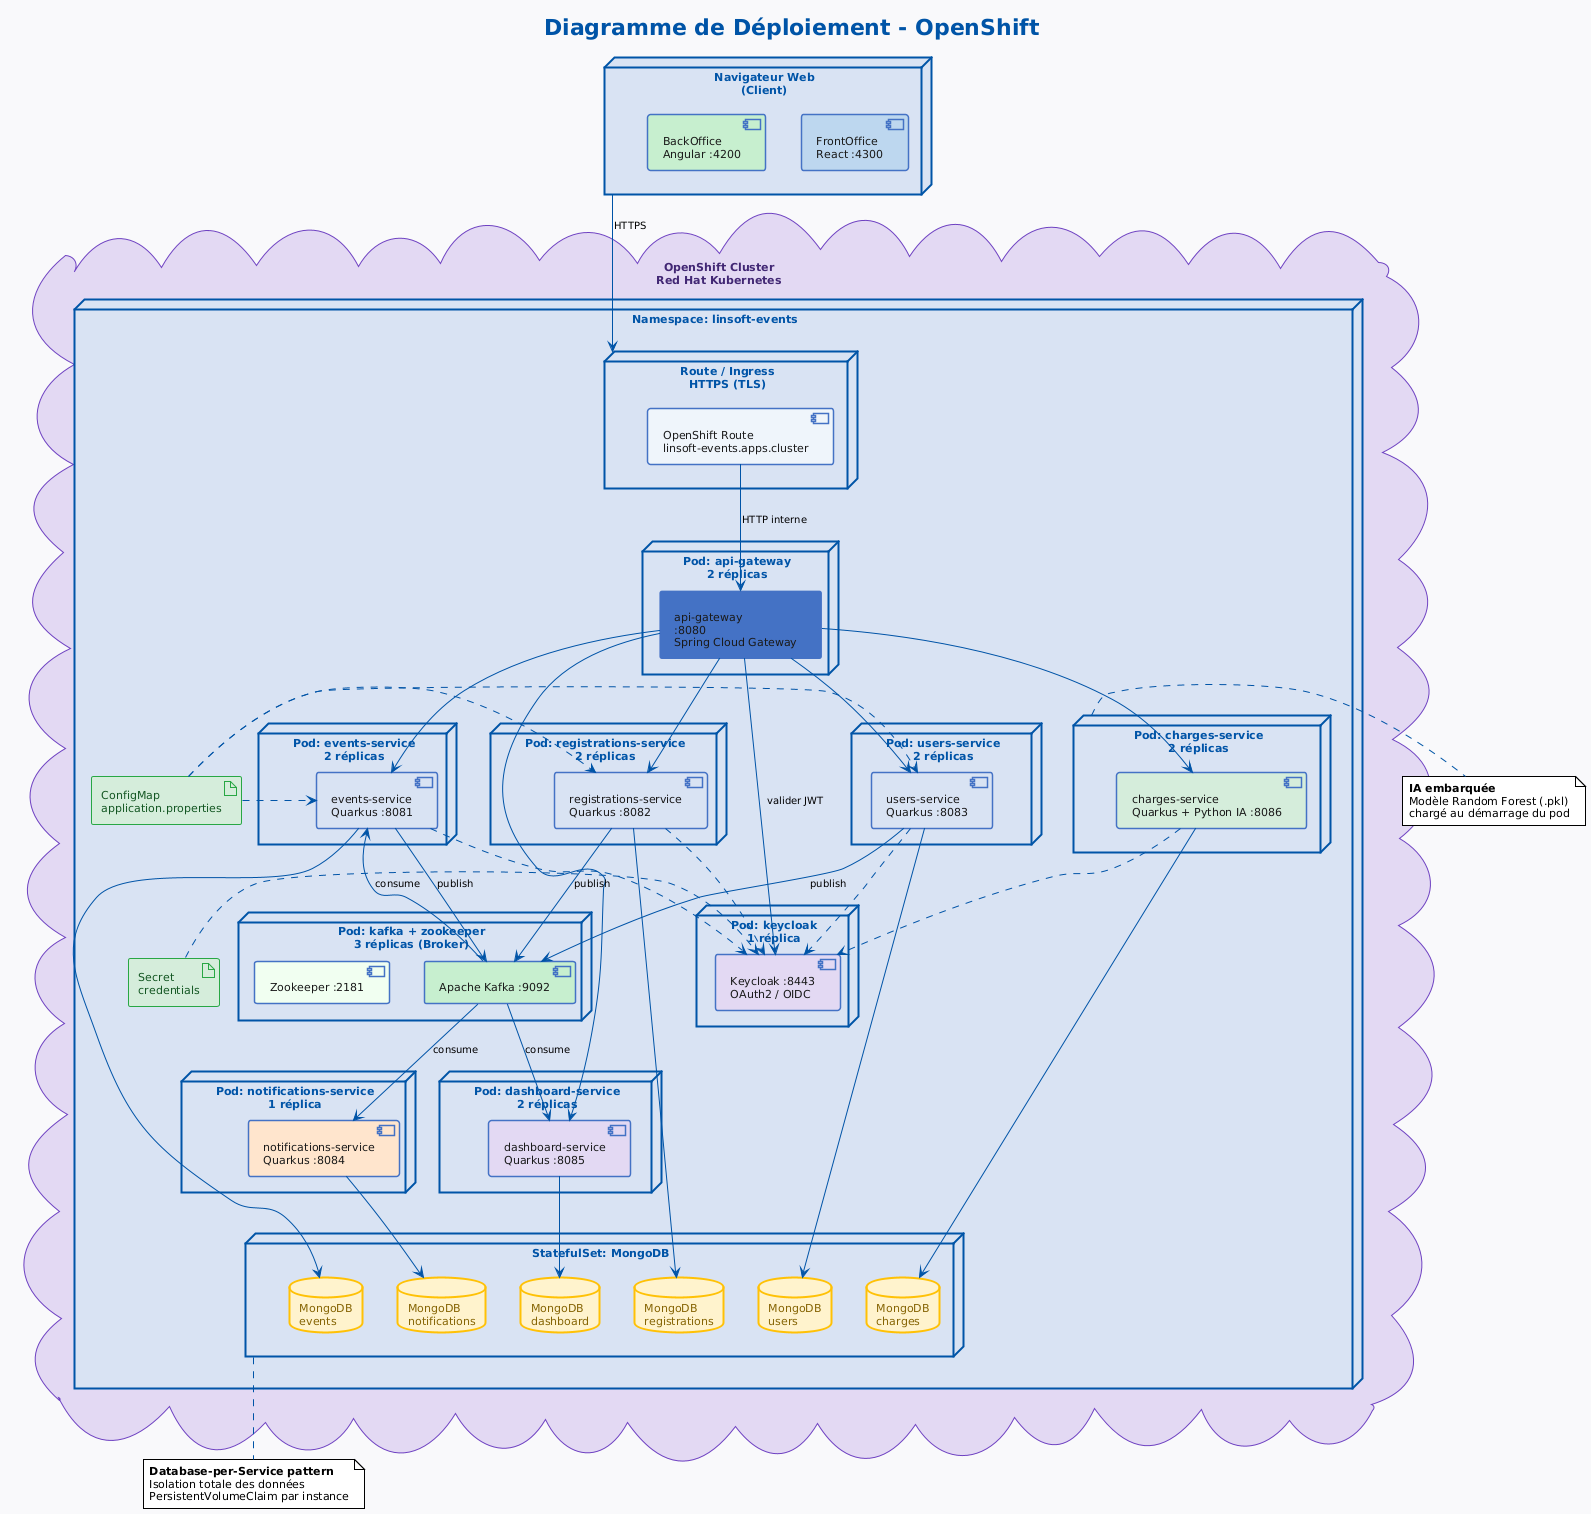
\includegraphics[width=\textwidth]{figures/deploiement.png}
\caption{Diagramme de d\'eploiement -- Namespace OpenShift linsoft-events}
\label{fig:deploiement}
\end{figure}

Chaque microservice est d\'eploy\'e avec : Deployment (2 r\'eplicas, RollingUpdate),
Service ClusterIP, Route HTTPS, ConfigMap, Secrets et Health Probes (/q/health).

\section*{Conclusion}
\addcontentsline{toc}{section}{Conclusion}

Ce chapitre a pr\'esent\'e la r\'ealisation compl\`ete : APIs, tests, captures
d'\'ecran de validation et d\'eploiement OpenShift. La plateforme r\'epond
int\'egralement aux besoins identifi\'es au chapitre~1, avec une architecture
scalable, s\'ecuris\'ee et maintenue en production.

%==================================================================
\chapter*{Conclusion G\'en\'erale}
\addcontentsline{toc}{chapter}{Conclusion G\'en\'erale}
%==================================================================

Ce projet de fin d'\'etudes a abouti \`a la conception et au d\'eveloppement complet
d'une plateforme cloud-native de gestion d'\'ev\'enements pour LinSoft. Construit
autour de six microservices Quarkus communiquant via REST et Apache Kafka, le
syst\`eme int\`egre une authentification centralis\'ee Keycloak, un pipeline de
pr\'ediction des co\^uts par intelligence artificielle (Random Forest, $R^2 = 0{,}91$)
et un d\'eploiement automatis\'e sur OpenShift Red Hat.

Les principaux apports de ce travail sont les suivants. D'abord, la plateforme
r\`egle les probl\`emes op\'erationnels concrets de LinSoft : inscriptions en ligne,
notifications automatis\'ees, gestion structur\'ee des charges et pilotage budg\'etaire
pr\'edictif. Ensuite, l'architecture event-driven garantit la scalabilit\'e et le
d\'ecouplage des services, rendant le syst\`eme extensible sans refonte majeure.
Enfin, l'approche Scrum adopt\'ee a permis de livrer des incr\'ements fonctionnels
\`a chaque sprint, facilitant la validation continue avec l'encadrant technique.

Sur le plan personnel, ce projet a \'et\'e l'occasion de consolider des comp\'etences
en architecture distribu\'ee, en DevOps et en machine learning appliqu\'e, dans un
contexte professionnel exigeant qui correspond aux r\'ealit\'es du march\'e MEA.

Des perspectives d'am\'elioration existent : int\'egration d'un syst\`eme de paiement
en ligne, internationalisation de l'interface, et enrichissement du mod\`ele IA avec
des donn\'ees historiques plus larges pour am\'eliorer la pr\'ecision des pr\'edictions.

%==================================================================
% BIBLIOGRAPHIE
%==================================================================
\begin{thebibliography}{99}

\bibitem{quarkus}
Red Hat. \textit{Quarkus -- Supersonic Subatomic Java}.
\url{https://quarkus.io/guides/}. Consult\'e en 2025.

\bibitem{kafka}
Apache Software Foundation. \textit{Apache Kafka Documentation}.
\url{https://kafka.apache.org/documentation/}. Consult\'e en 2025.

\bibitem{keycloak}
Red Hat. \textit{Keycloak -- Open Source Identity and Access Management}.
\url{https://www.keycloak.org/documentation}. Consult\'e en 2025.

\bibitem{openshift}
Red Hat. \textit{OpenShift Container Platform Documentation}.
\url{https://docs.openshift.com/}. Consult\'e en 2025.

\bibitem{mongodb}
MongoDB Inc. \textit{MongoDB Manual}.
\url{https://www.mongodb.com/docs/manual/}. Consult\'e en 2025.

\bibitem{sklearn}
Pedregosa, F. et al. \textit{Scikit-learn: Machine Learning in Python}.
\textit{Journal of Machine Learning Research}, 12:2825--2830, 2011.

\bibitem{microservices}
Newman, S. \textit{Building Microservices: Designing Fine-Grained Systems}.
O'Reilly Media, 2nd edition, 2021.

\bibitem{evendriven}
Richardson, C. \textit{Microservices Patterns}.
Manning Publications, 2018.

\bibitem{docker}
Docker Inc. \textit{Docker Documentation}.
\url{https://docs.docker.com/}. Consult\'e en 2025.

\bibitem{angular}
Google. \textit{Angular Documentation}.
\url{https://angular.io/docs}. Consult\'e en 2025.

\bibitem{react}
Meta Open Source. \textit{React Documentation}.
\url{https://react.dev/}. Consult\'e en 2025.

\bibitem{jwt}
Jones, M. et al. \textit{JSON Web Token (JWT) -- RFC 7519}.
\url{https://www.rfc-editor.org/rfc/rfc7519}. 2015.

\end{thebibliography}

\end{document}
igning Fine-Grained Systems}.
O'Reilly Media, 2nd edition, 2021.

\bibitem{evendriven}
Richardson, C. \textit{Microservices Patterns}.
Manning Publications, 2018.

\bibitem{docker}
Docker Inc. \textit{Docker Documentation}.
\url{https://docs.docker.com/}. Consult\'e en 2025.

\bibitem{angular}
Google. \textit{Angular Documentation}.
\url{https://angular.io/docs}. Consult\'e en 2025.

\bibitem{react}
Meta Open Source. \textit{React Documentation}.
\url{https://react.dev/}. Consult\'e en 2025.

\bibitem{jwt}
Jones, M. et al. \textit{JSON Web Token (JWT) -- RFC 7519}.
\url{https://www.rfc-editor.org/rfc/rfc7519}. 2015.

\end{thebibliography}

\end{document}
